%%%%%%%%%%%%%%%%%%%%%%%%%%%%%%%%%%%%%%%%%%%%%%%%%%%%%%
% A Beamer template for University of Wollongong     %
% Based on THU beamer theme                          %
% Author: Qiuyu Lu                                   %
% Date: July 2024                                    %
% LPPL Licensed.                                     %
%%%%%%%%%%%%%%%%%%%%%%%%%%%%%%%%%%%%%%%%%%%%%%%%%%%%%%
% Customized for Sharif University of Technology     %
%%%%%%%%%%%%%%%%%%%%%%%%%%%%%%%%%%%%%%%%%%%%%%%%%%%%%%


\documentclass[serif, aspectratio=169]{beamer}
%\documentclass[serif]{beamer}  % for 4:3 ratio
\usepackage[T1]{fontenc} 
\usepackage{fourier} % see "http://faq.ktug.org/wiki/uploads/MathFonts.pdf" for other options
\usepackage{hyperref}
\usepackage{latexsym,amsmath,xcolor,multicol,booktabs,calligra}
\usepackage{graphicx,listings,stackengine}
\usepackage{lipsum}
\usepackage{tikz}


\author{Ali Sharifi-Zarchi}
% \author{CE Department}
\title{Machine Learning (CE 40477)}
\subtitle{Fall 2025}
\institute{
    CE Department \\
    Sharif University of Technology
}
\usepackage{SUTstyle}

% defs
\def\cmd#1{\texttt{\color{red}\footnotesize $\backslash$#1}}
\def\env#1{\texttt{\color{blue}\footnotesize #1}}
\definecolor{deepblue}{rgb}{0,0,0.5}
\definecolor{deepred}{RGB}{153,0,0}
\definecolor{deepgreen}{rgb}{0,0.5,0}
\definecolor{halfgray}{gray}{0.55}

\lstset{
    basicstyle=\ttfamily\small,
    keywordstyle=\bfseries\color{deepblue},
    emphstyle=\ttfamily\color{deepred},    % Custom highlighting style
    stringstyle=\color{deepgreen},
    numbers=left,
    numberstyle=\small\color{halfgray},
    rulesepcolor=\color{red!20!green!20!blue!20},
    frame=shadowbox,
}

\begin{document}

\begin{frame}
    \titlepage
    \vspace*{-0.6cm}
    \begin{figure}[htpb]
    \begin{center}
        
\includegraphics[keepaspectratio, scale=0.25]{pic/sharif-main-logo.png}
    \end{center}
\end{figure}

\end{frame}


\begin{frame}{Teaching Team}
\textbf{Teaching Team}
\begin{itemize}
    \item \textbf{Instructor:} Dr. Ali Sharifi Zarchi \\
          \href{mailto:asharifi@sharif.edu}{asharifi@sharif.edu} \\
          \href{mailto:asharifiz@gmail.com}{asharifiz@gmail.com}
    \item \textbf{Team Captain:} Alireza Mirrokni \\
          \href{mailto:alirezamirrokni28@gmail.com}{alirezamirrokni28@gmail.com}
\end{itemize}


\end{frame}


\begin{frame}{Course Overview}
\textbf{Course Overview}
\begin{itemize}
    \item Supervised Learning
    \item Unsupervised Learning
    \item Neural Networks
    \item Computer Vision
    \item Natural Language Processing
    \item Additional Chapter (Agentic AI)
\end{itemize}
\end{frame}




\begin{frame}{Supervised Learning}
\textbf{Learn to predict outcomes using labeled data.}

\begin{itemize}
    \item Predict house prices from past sales data.
    \item Use features such as size, location, and room count.
\end{itemize}


\begin{center}
    \centering
    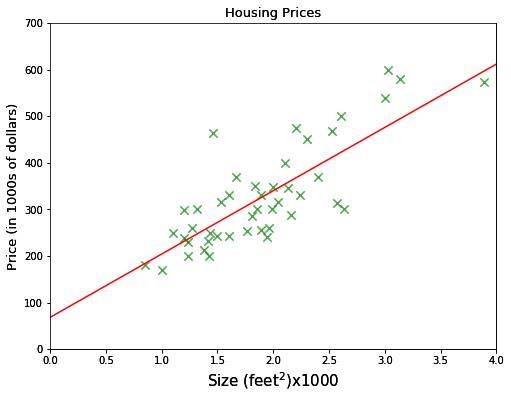
\includegraphics[width=0.4\linewidth]{pic/be1.jpg}
\end{center}

\textbf{Learn More:}
\href{https://towardsdatascience.com/predicting-house-prices-with-linear-regression-machine-learning-from-scratch-part-ii-47a0238aeac1}{Predicting House Prices with Linear Regression}
\end{frame}

\begin{frame}{Unsupervised Learning}
\textbf{Discover hidden structures within unlabeled data.}

\begin{itemize}
    \item Identify groups or patterns without predefined labels.
\end{itemize}

\begin{center}
    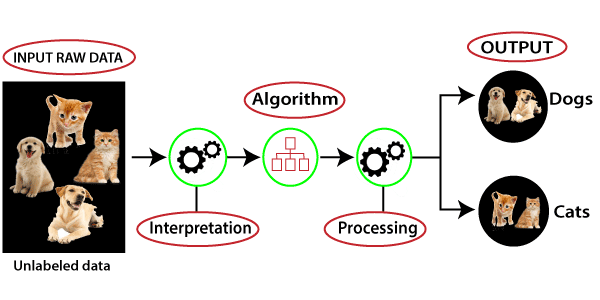
\includegraphics[width=0.7\linewidth]{pic/be2.png}
\end{center}

\begin{center}
\textit{Example: Image clustering.}
\end{center}
\end{frame}



\begin{frame}{Neural Networks}
    \begin{itemize}
        \item Designed to mimic the human brain in order to solve complex tasks
    \end{itemize}
    \vspace{0.4cm}
    \begin{center}
        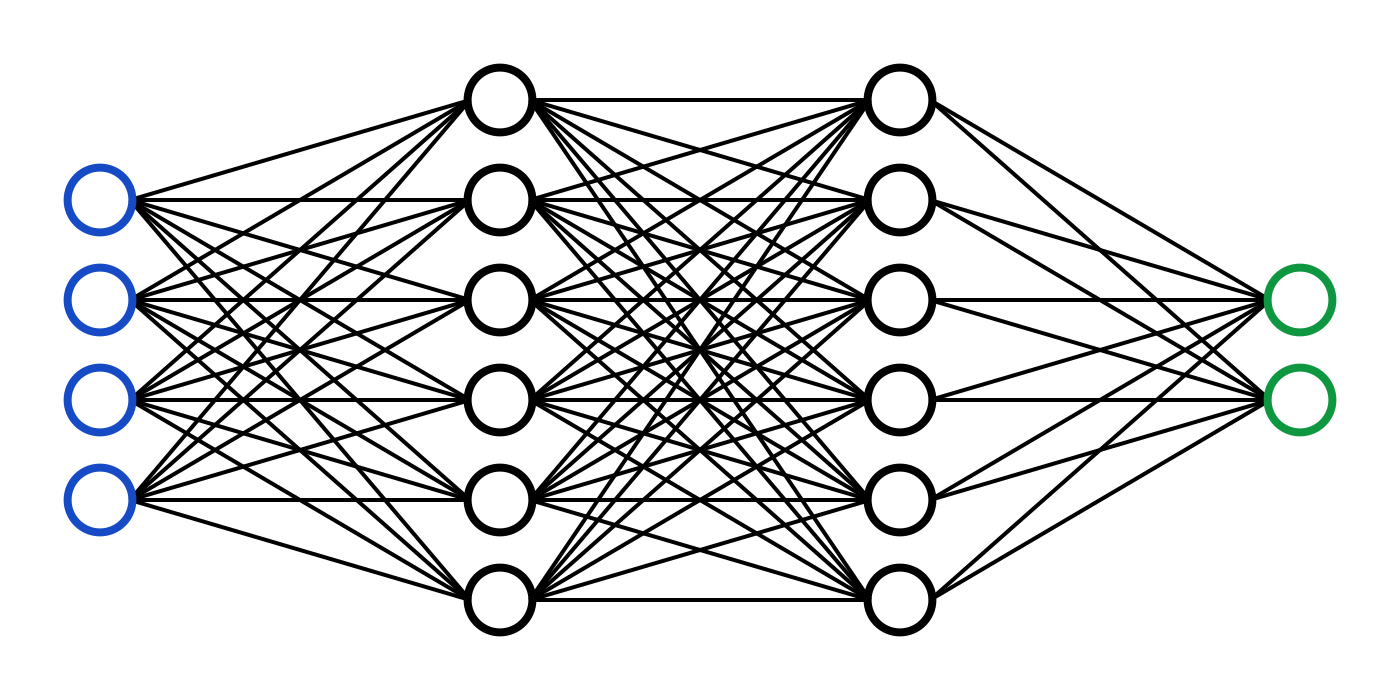
\includegraphics[width=0.7\linewidth]{pic/be3.png}
    \end{center}
    \vspace{0.3cm}
    \begin{center}
        \textit{Examples: Facial recognition, voice assistants.}
    \end{center}
\end{frame}

\begin{frame}{Computer Vision}
    \begin{itemize}
        \item Enables machines to perceive and interpret visual information
    \end{itemize}
    \begin{center}
        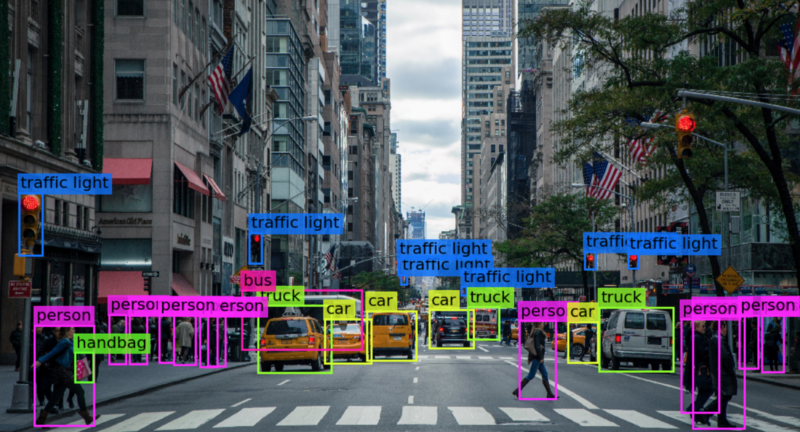
\includegraphics[width=0.7\linewidth]{pic/be4.png}
    \end{center}
    \begin{center}
        \textit{Examples: Factory quality control, medical image analysis.}
    \end{center}
\end{frame}


\begin{frame}{Natural Language Processing (NLP)}
    \begin{itemize}
        \item Understand and generate human language
    \end{itemize}
    \vspace{0.5cm}
    \begin{center}
        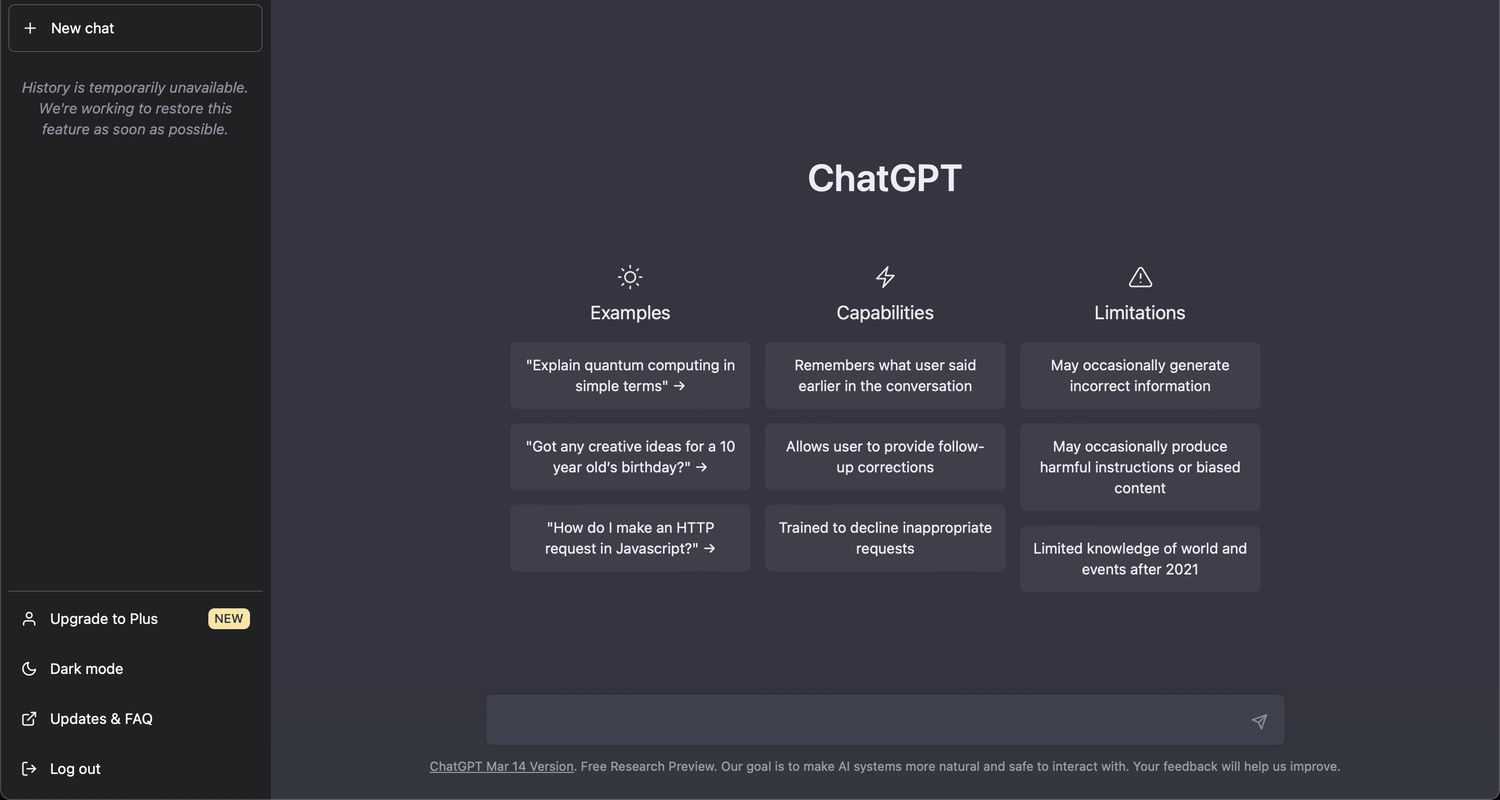
\includegraphics[width=0.6\linewidth]{pic/be5.png}
    \end{center}
    % \vspace{0.5cm}
    \begin{center}
        \textit{Example: Chat-bots, language translation.}
    \end{center}
\end{frame}





\begin{frame}{What is Machine Learning (ML)?}
    \begin{itemize}
        \item \textbf{Machine Learning}: Enables computers to learn patterns from data without explicit programming.
        \item Focuses on predicting outcomes, classification, or discovering hidden structures.
    \vspace{4mm}

        \item \textbf{Goal}: Build models that make accurate predictions from past data.
    \end{itemize}
\end{frame}



\begin{frame}{Tom M. Mitchell's Definition of ML}
    \begin{quote}
    "A computer program is said to learn from experience $E$ with respect to some class of tasks $T$ and performance measure $P$, if its performance at tasks in $T$, as measured by $P$, improves with experience $E$."
    \end{quote}
    \vspace{2mm}
    \begin{itemize}
        \item Formally: $\text{Learning Problem} = (T, P, E)$
        \item Example: Predicting house prices using past data.
    \end{itemize}
\end{frame}




\begin{frame}{Paradigms of ML}

\begin{minipage}{1.0\textwidth}
    \begin{itemize}
        \item \textbf{Supervised learning} (regression, classification)
        \begin{itemize}
            \item predicting a target variable for which we get to see examples.
        \end{itemize}
        \item \textbf{Unsupervised learning}
        \begin{itemize}
            \item revealing structure in the observed data
        \end{itemize}
        \item \textbf{Reinforcement learning}
        \begin{itemize}
            \item partial (indirect) feedback, no explicit guidance
            \item given rewards for a sequence of moves to learn a policy and utility functions
        \end{itemize}
        \item \textbf{Other paradigms:} semi-supervised learning, active learning, online learning, etc.
    \end{itemize}
\end{minipage}%
\end{frame}





\begin{frame}{Supervised Learning}
    \begin{itemize}
        \item \textbf{Definition}: A form of machine learning where the model learns from labeled data \( \{(x_i, y_i)\} \) to predict an output \( y \) given an input \( x \).
        \item \textbf{Goal}: Estimate a function \( f: \mathbb{R}^D \rightarrow \mathbb{R} \), such that \( y = f(x) + \epsilon \), where \( \epsilon \) is noise.
    \end{itemize}
     \begin{center}
        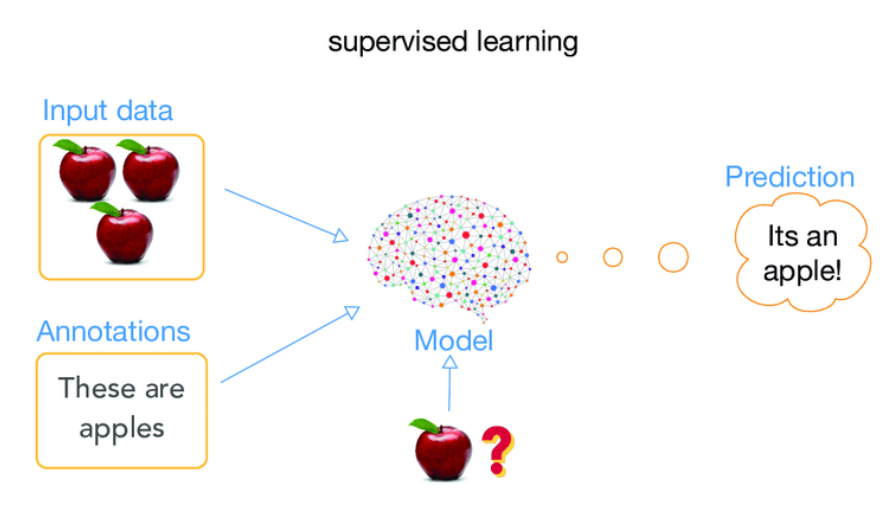
\includegraphics[width=0.6\linewidth]{pic/supervised.png}
    \end{center}
\end{frame}

\begin{frame}
    \frametitle{Components of (Supervised) Learning}

    \begin{itemize}
        \item \textbf{Unknown target function:} \( f : \mathcal{X} \to \mathcal{Y} \)
        \begin{itemize}
            \item \textbf{Input space:} \( \mathcal{X} \)
            \item \textbf{Output space:} \( \mathcal{Y} \)
        \end{itemize}

        \vspace{0.5cm} % for spacing between points

        \item \textbf{Training data:} \( (x_1, y_1), (x_2, y_2), \ldots, (x_N, y_N) \)

        \vspace{0.5cm}

        \item \textbf{Pick a formula} \( g : \mathcal{X} \to \mathcal{Y} \) \textbf{that approximates the target function} \( f \)
        \begin{itemize}
            \item selected from a set of hypotheses \( \mathcal{H} \)
        \end{itemize}
    \end{itemize}

\end{frame}


\begin{frame}{Components of (Supervised) Learning (cont.)}
    \begin{minipage}{0.95\textwidth}
        \begin{figure}[h]
          \centering
          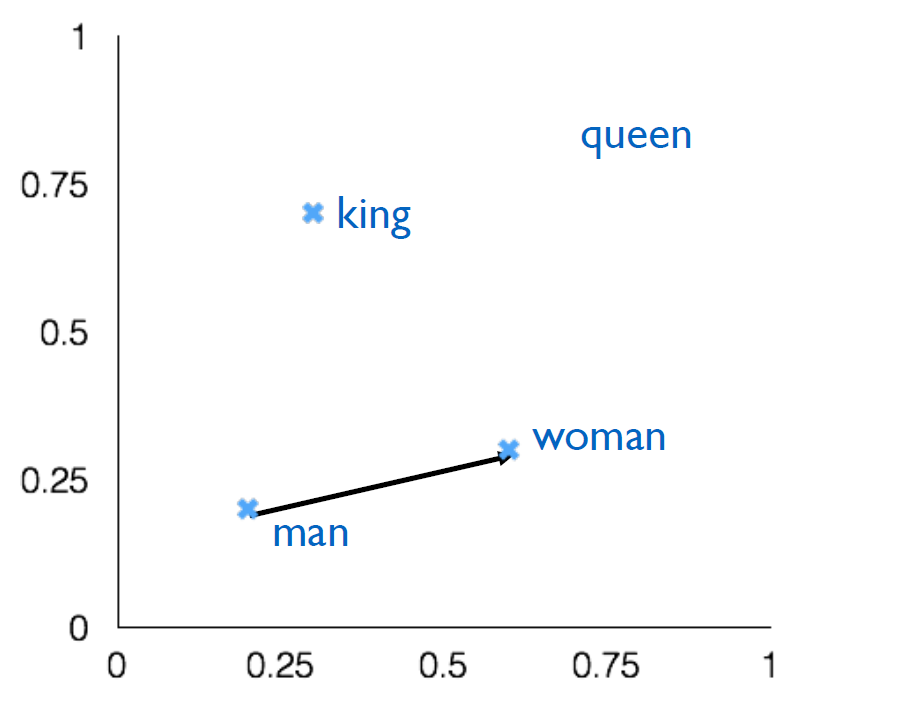
\includegraphics[width=0.7\linewidth]{pic/4.png}
        \end{figure}
    \end{minipage}
    \vfill
    \begin{tikzpicture}[remember picture,overlay]
        \node[anchor=south west, xshift=0.1cm, yshift=0.22cm] at (current page.south west) {
            \tiny Figure adapted from Abu-Mostafa, Yaser S., Malik Magdon-Ismail, and Hsuan-Tien Lin. Learning from Data: A Short Course
        };
    \end{tikzpicture}
\end{frame}



\begin{frame}{Supervised Learning: Regression vs. Classification}

    \begin{itemize}
        \item \textbf{Regression}: predict a \underline{continuous} target variable
        \begin{itemize}
            \item E.g., $y \in [0, 1]$
        \end{itemize}
        \item \textbf{Classification}: predict a \underline{discrete} target variable
        \begin{itemize}
            \item E.g., $y \in \{1, 2, \ldots, C\}$
        \end{itemize}
    \end{itemize}

        \centering
        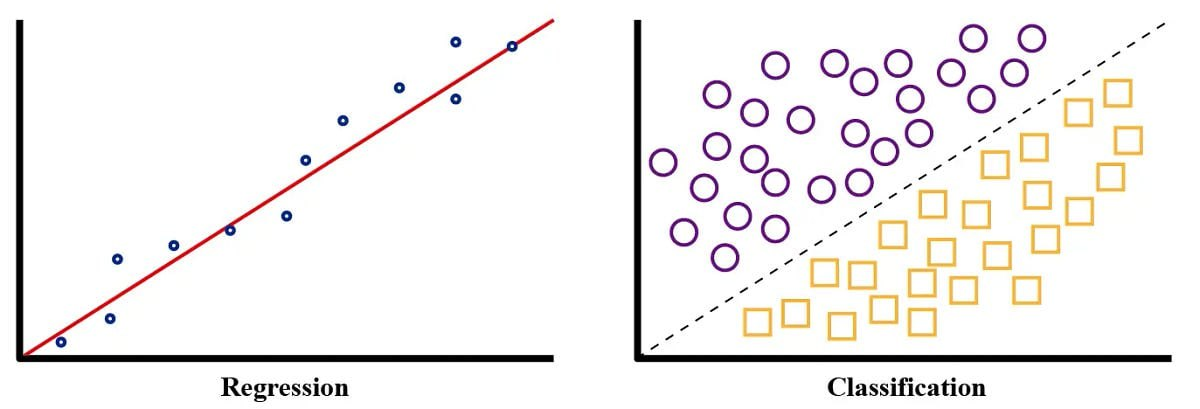
\includegraphics[width=0.8\linewidth]{pic/regressionVSclassification.jpg}



\end{frame}



\begin{frame}{Solution Components - Learning Model}
    \begin{itemize}
        \item The \textbf{Learning Model} consists of:
        \begin{itemize}
            \item \textbf{Hypothesis Set}: Defines the possible functions \( \mathcal{H} = \{h(x, \theta) | \theta \in \Theta\} \), where \( h(x, \theta) \) represents candidate functions and \( \theta \) is the learning parameters of problem.
            \item \textbf{Learning Algorithm}: Find \( \theta^* \in \Theta \) such that \( h(x, \theta^*) \approx f(x) \).
        \end{itemize}
        \item Both work together to map inputs \(x\) to outputs \(y\) with minimized error.
        \item In other words, \( \theta^* \) is best parameters to predict outputs using chosen hypothesis.
    \end{itemize}
    \vspace{0.5cm}
\end{frame}




\begin{frame}{Hypothesis Space Overview}
    \begin{itemize}
        \item \textbf{Hypothesis (h)}: A mapping from input space \( \mathcal{X} \) to output space \( \mathcal{Y} \).
        \item \textbf{Linear Regression Hypothesis}:
        \[
        h_{\mathbf{w}}(\mathbf{x}) = w_0 + w_1 x_1 + \dots + w_D x_D = \mathbf{w}^\top \mathbf{x}
        \]
        \item \textbf{Input Vector} \( \mathbf{x} \):
        \[
        \mathbf{x} = \begin{bmatrix} x_0 = 1, x_1, x_2, \dots, x_D \end{bmatrix}
        \]
        \item \textbf{Parameter Vector} \( \mathbf{w} \):
        \[
        \mathbf{w} = \begin{bmatrix} w_0, w_1, w_2, \dots, w_D \end{bmatrix}
        \]
    \end{itemize}
\end{frame}





\begin{frame}{Linear Hypothesis Representation}
    \begin{itemize}
        \item \textbf{Linear Hypothesis Space}:
        \begin{itemize}
            \item \textbf{Simplest form}: Linear combination of input features.
            \[
            h_{\mathbf{w}}(\mathbf{x}) = w_0 + \sum_{i=1}^{D} w_i x_i
            \]
        \end{itemize}
        \item \textbf{Linear Hypothesis Examples}:
        \begin{itemize}
            \item \textbf{Single Variable}: \( h_{\mathbf{w}}(x) = w_0 + w_1 x \)
            \item \textbf{Multivariate}: \( h_{\mathbf{w}}(\mathbf{x}) = w_0 + w_1 x_1 + w_2 x_2 + ... + w_D x_D \)
        \end{itemize}
    \end{itemize}
\end{frame}


\begin{frame}{Understanding Cost Functions}
    \begin{itemize}
        \item In \textbf{hypothesis space}, we select a function \( h(x; \mathbf{w}) \) to approximate the true relationship between input \( x \) and output \( y \).
        \item The objective is to minimize the difference between predicted values \( h(x) \) and actual values \( y \).
        \item This difference is quantified using \textbf{cost functions}, which guide us in choosing the optimal hypothesis.
    \end{itemize}
\end{frame}


\begin{frame}{What is a Cost Function?}
    \begin{itemize}
        \item A \textbf{cost function} measures how well the hypothesis \( h(x; \mathbf{w}) \) fits the training data.
        \item In regression problems, the most common error function is the \textbf{Squared Error (SE)}:
            \[
            SE: \left( y^{(i)} - h(x^{(i)}; \mathbf{w}) \right)^2
            \]
        \item Cost function should measure all predictions. Thus a choice could be \textbf{Sum of Squared Errors (SSE)}:
        \[
        J(\mathbf{w}) = \sum_{i=1}^{N} \left( y^{(i)} - h(x^{(i)}; \mathbf{w}) \right)^2
        \]
        \item \textbf{Objective:} Minimize the cost function to find the best parameters \( \mathbf{w} \).

    \end{itemize}

\end{frame}

\begin{frame}{SSE: Sum of Squared Errors}
    \begin{itemize}
        \item \textbf{SSE} is widely used due to its simplicity and differentiability.
        \item Intuitively, it represents the squared distance between predicted and true values.
        \item Penalizes larger errors more severely than smaller ones (due to the square).
        \item For linear regression, it can be written as:
        \[
        SSE = \sum_{i=1}^{N} \left( y^{(i)} - \mathbf{w}^T \mathbf{x}^{(i)} \right)^2
        \]
    \end{itemize}
\end{frame}





\begin{frame}{How to measure the error}

    \begin{minipage}{0.5\textwidth}
        \centering
        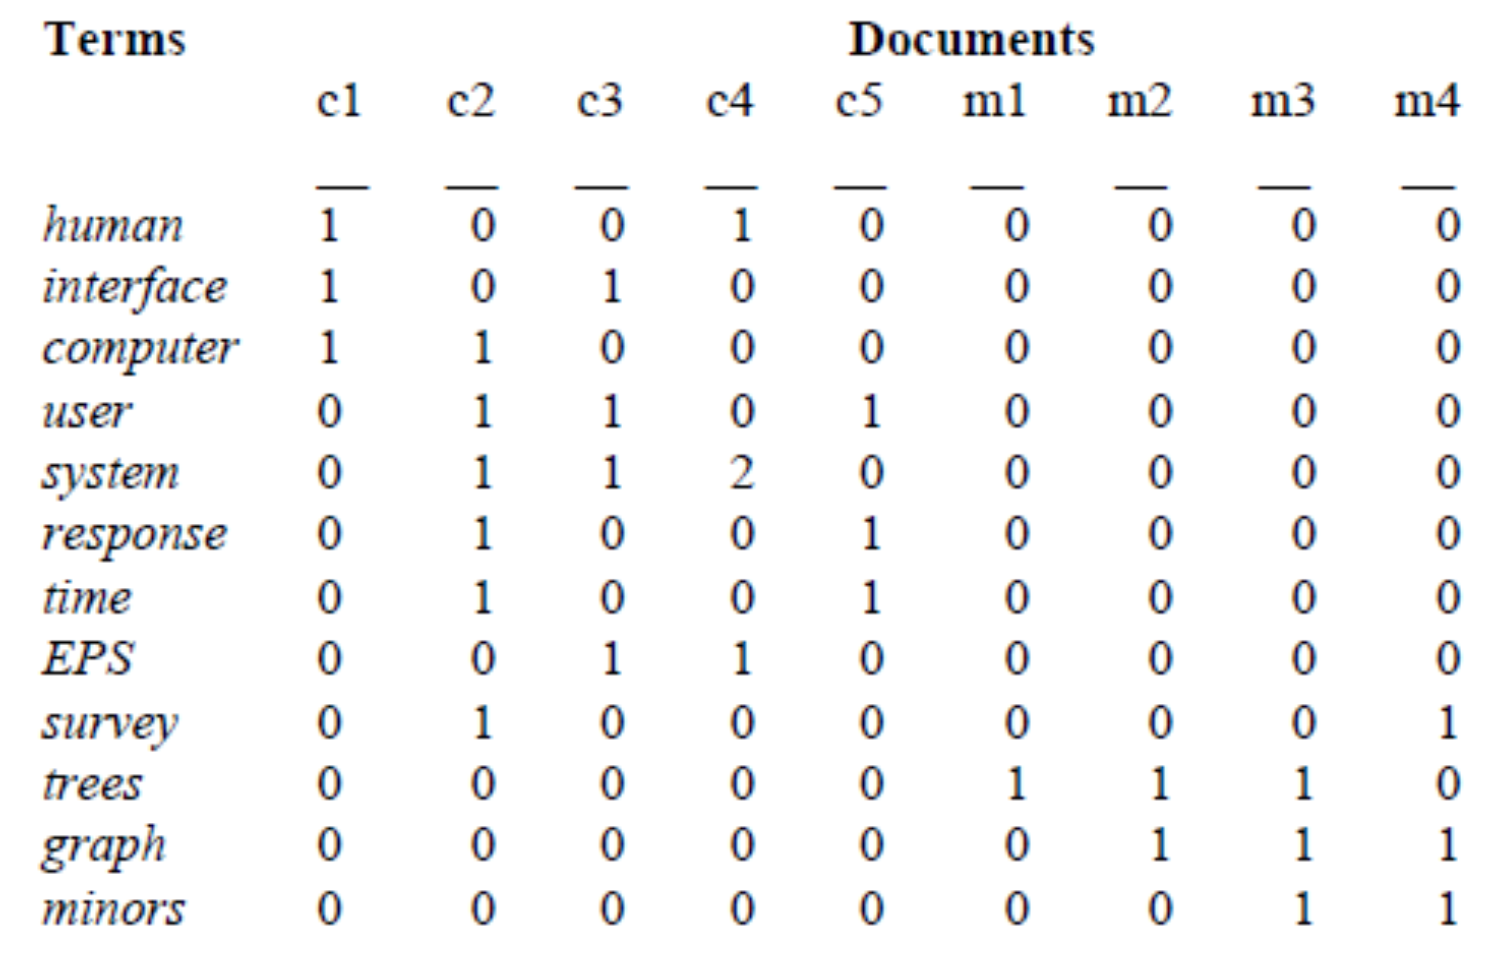
\includegraphics[width=\textwidth]{pic/6.png}
    \end{minipage}%
    \begin{minipage}{0.5\textwidth}

        \[
        J(w) = \sum_{i=1}^{n} \left( y^{(i)} - h_w(x^{(i)}) \right)^2
        \]
        \[
        = \sum_{i=1}^{n} \left( y^{(i)} - w_0 - w_1 x^{(i)} \right)^2
        \]
    \end{minipage}
    \vfill
    \begin{tikzpicture}[remember picture,overlay]
        \node[anchor=south west, xshift=0.1cm, yshift=0.22cm] at (current page.south west) {
            \scriptsize Figure adapted from slides of Dr. Soleymani, Machine Learning course, Sharif university of technology.
        };
    \end{tikzpicture}
\end{frame}


\begin{frame}{The learning algorithm}

    \begin{itemize}
        \item \textbf{Objective:} Choose \( \mathbf{w} \) so as to minimize the \( J(\mathbf{w}) \)
        % \[
        % J(w) = \sum_{i=1}^{n} \left( y^{(i)} - h_w(x^{(i)}) \right)^2
        % \]

        \item \textbf{The learning algorithm:} optimization of the cost function
        \begin{itemize}
            \item Explicitly taking the cost function derivative with respect to the \( w_i \)'s, and setting them to zero.
        \end{itemize}

        \item Parameters of the best hypothesis for the training set:
        \[
        w^* = \arg \min_{w} J(w)
        \]
    \end{itemize}


\end{frame}




\begin{frame}{Cost function optimization: univariate}
    \[
    J(w) = \sum_{i=1}^{n} \left( y^{(i)} - w_0 - w_1 x^{(i)} \right)^2
    \]

    \begin{itemize}
        \item \textbf{Necessary conditions for the “optimal” parameter values:}
        \[
        \frac{\partial J(w)}{\partial w_0} = 0, \qquad
        \frac{\partial J(w)}{\partial w_1} = 0
        \]

    \[
    \frac{\partial J(w)}{\partial w_1} = \sum_{i=1}^{n} 2 \left( y^{(i)} - w_0 - w_1 x^{(i)} \right) (-x^{(i)}) = 0
    \]

    \[
    \frac{\partial J(w)}{\partial w_0} = \sum_{i=1}^{n} 2 \left( y^{(i)} - w_0 - w_1 x^{(i)} \right) (-1) = 0
    \]

    \begin{itemize}
        \item A system of 2 linear equations
    \end{itemize}
    \end{itemize}


\end{frame}





\begin{frame}{Linear regression example: TV Advertising and Sales}
    This is a real-world example of how businesses can use linear regression to make decisions about marketing budgets. The following table shows the amount of TV advertising budget spend and respective average sales of houses in Boston:
    \begin{table}[h!]
    \centering
    \begin{tabular}{|c|c|}
    \hline
    \textbf{TV Advertising Spend (\$1000)} & \textbf{Sales (Units)} \\ \hline
    230.1                                  & 22.1                   \\ \hline
    44.5                                   & 10.4                   \\ \hline
    17.2                                   & 9.3                    \\ \hline
    151.5                                  & 18.5                   \\ \hline
    180.8                                  & 12.9                   \\ \hline
    \end{tabular}
    \caption{TV Advertising Spend vs. Sales Dataset}
    \end{table}

\textbf{Learn More:}
\href{https://www.kaggle.com/datasets/yasserh/advertising-sales-dataset}{Advertising Sales Dataset}
\end{frame}





\begin{frame}{Linear regression example: TV Advertising and Sales (cont.)}
    \begin{itemize}
        \item In this problem, Sales per TV advertising is need thus the amount spend is considered as input \( x \) and sales is considered as output \( y \).
        \item Using linear regression, cost function can be written as:
        \[
        J(w) = \sum_{i=1}^{5} \left( y^{(i)} - w_0 - w_1 x^{(i)} \right)^2
        \]
        \item Applying necessary conditions for the optimal parameters:
        \[
        \frac{\partial J(w)}{\partial w_1} = \sum_{i=1}^{5} 2 \left( y^{(i)} - w_0 - w_1 x^{(i)} \right) (-x^{(i)}) = 0 \implies 110863 w_1 + 624.1 w_0 - 10843.04 = 0
        \]
        \[
        \frac{\partial J(w)}{\partial w_0} = \sum_{i=1}^{5} 2 \left( y^{(i)} - w_0 - w_1 x^{(i)} \right) (-1) = 0 \implies 624.1 w_1 + 5 w_0 - 73.2 = 0
        \]
    \end{itemize}
\end{frame}





\begin{frame}{Linear regression example: TV Advertising and Sales (cont.)}
\begin{minipage}{0.4\textwidth}
    \begin{itemize}
        \item Solving the system of two equations described, we get:
        \[ w_1 \approx 0.052 \]
        \[ w_0 \approx 8.18 \]
    \end{itemize}
\end{minipage}%
\begin{minipage}{0.55\textwidth}
\centering
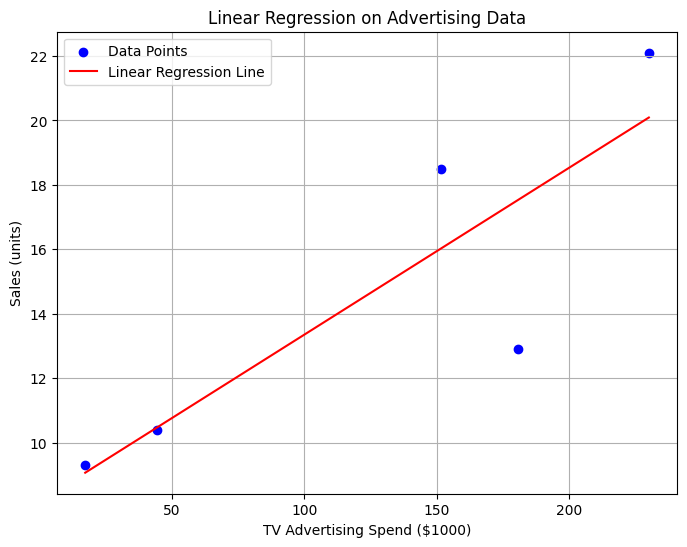
\includegraphics[width=0.75\textwidth]{pic/boston.png}
\end{minipage}

\end{frame}

\begin{frame}{Cost function optimization: multivariate}
    \begin{itemize}
        \item Remembering \textbf{SSE cost function} of multivariate linear regression
            \[
            J(w) = \sum_{i=1}^{n} \left( y^{(i)} - h_w(x^{(i)}) \right)^2 = \sum_{i=1}^{n} \left( y^{(i)} - \mathbf{w}^T \mathbf{x}^{(i)} \right)^2
            \]
        \item We usually write matrix form of the problem as follows:

    \end{itemize}

    \[
    \mathbf{X} =
    \begin{bmatrix}
    1 & x_1^{(1)} & \cdots & x_d^{(1)} \\
    1 & x_1^{(2)} & \cdots & x_d^{(2)} \\
    \vdots & \vdots & \ddots & \vdots \\
    1 & x_1^{(n)} & \cdots & x_d^{(n)}
    \end{bmatrix}
    \quad
    \mathbf{w} =
    \begin{bmatrix}
    w_0 \\
    w_1 \\
    \vdots \\
    w_d
    \end{bmatrix}
    \quad
    \mathbf{y} =
    \begin{bmatrix}
    y^{(1)} \\
    \vdots \\
    y^{(n)}
    \end{bmatrix}
    \]

    \begin{center}
    In which \( x_m^{(i)} \) indicates \(m \)'th feature of data point \( i\) \\
    \end{center}

\end{frame}

\begin{frame}{Cost function optimization: multivariate}

    \begin{itemize}
        \item Using the matrix forms suggested, we can rewrite cost function:
        \[
        J(\mathbf{w}) = \| \mathbf{y} - \mathbf{Xw} \|_2^2
        \]
        \item Explicitly taking the cost function derivative with respect to the \( \mathbf{w} \), and setting them to zero:
        \[
        \nabla_w J(\mathbf{w}) = -2 \mathbf{X}^T \left( \mathbf{y} - \mathbf{Xw} \right)
        \]
        \[
        \nabla_w J(\mathbf{w}) = 0 \implies \mathbf{X}^T \mathbf{Xw} = \mathbf{X}^T \mathbf{y} \implies \mathbf{w} = \left( \mathbf{X}^T \mathbf{X} \right)^{-1} \mathbf{X}^T \mathbf{y}
        \]
    \end{itemize}

    % \begin{itemize}
    %     \item \textbf{Is} \( \mathbf{X}^T \mathbf{X} \) \textbf{invertible?}
    % \end{itemize}

    \begin{itemize}
        \item \( \left(\mathbf{X}^T \mathbf{X} \right)^{-1} \mathbf{X}^T \) is called pseudo-inverse of matrix \( \mathbf{X} \)
        \item The matrix \( \mathbf{X} \) is often not square yet not invertible. \item The pseudo-inverse can be computed for any matrix, regardless of its shape.
    \end{itemize}
\end{frame}

\begin{frame}{Computational limitations of analytical solution}
    \begin{itemize}
        \item \textbf{Scalability:} Analytical solutions do not scale well with very large datasets, making them impractical for big data applications.
        \item \textbf{Finding the inverse of a matrix:}
        \begin{itemize}
            \item Simplest way of finding inverse: Gaussian elimination, having complexity of \(O(n^3)\).
            \item Other methods: LU decomposition, which also has a complexity of \(O(n^3)\) but is more stable.
            \item Numerical methods: Iterative methods like Conjugate Gradient, which can be more efficient for large, sparse matrices.
        \end{itemize}
        % \item \textbf{Memory usage:} Storing large matrices in memory can be prohibitive, especially for very large datasets.
    \end{itemize}
\end{frame}

\begin{frame}{Practical limitations of analytical solution}

    \begin{itemize}
        \item \textbf{Online learning:} Data observations are arriving in a continuous stream
        \begin{itemize}
            \item Predictions must be made before seeing all of the data.
            \item Analytical solutions require all data to be available upfront, which is not feasible in online learning scenarios.
            \item Analytical methods are not adaptable to new data without re-computing the entire solution.
        \end{itemize}
    \end{itemize}

    \centering
    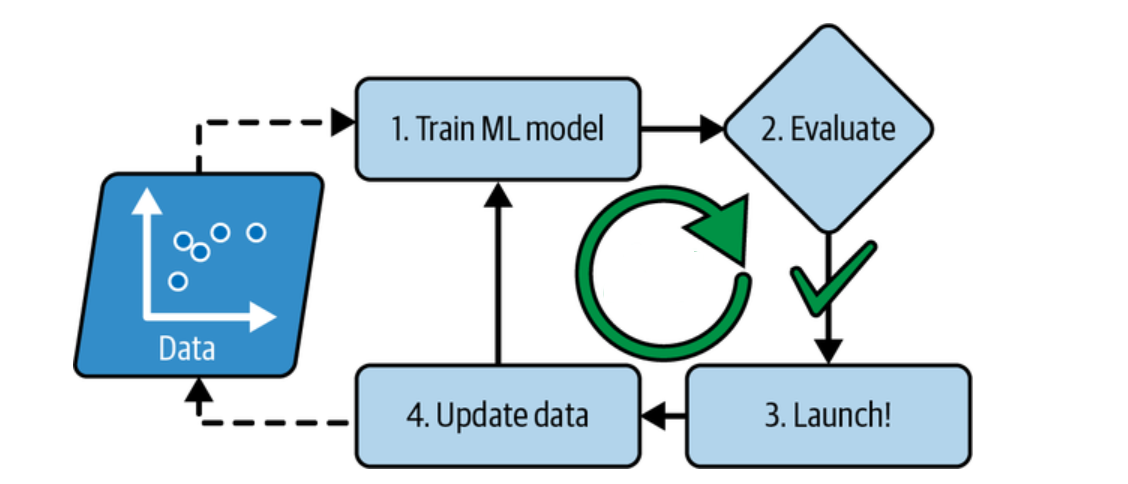
\includegraphics[width=0.6\linewidth]{pic/online-learning.png}

\end{frame}


\begin{frame}{Cost function optimization}

\begin{itemize}
    \item \textbf{Another approach,}
    \begin{itemize}
        \item Start from an initial guess and iteratively change \( w \) to minimize \( J(w) \).
        \begin{itemize}
            \item The gradient descent algorithm
        \end{itemize}
    \end{itemize}

    \item \textbf{Steps:}
    \begin{itemize}
        \item Start from \( w^0 \)
        \item Repeat:
        \begin{itemize}
            \item Update \( w^t \) to \( w^{t+1} \) in order to reduce \( J \)
            \item \( t \leftarrow t + 1 \)
        \end{itemize}
        until we hopefully end up at a minimum.
    \end{itemize}
\end{itemize}

\end{frame}



\begin{frame}{Gradient Descent}

    \begin{itemize}
        \item In each step, takes steps proportional to the negative of the gradient vector of the function at the current point \( w^t \):

        \[
        w^{t+1} = w^t - \eta \nabla J(w^t)
        \]

        \item \( J(w) \) \textbf{decreases fastest} if one goes from \( w^t \) in the direction of \( -\nabla J(w^t) \)

        \item \textbf{Assumption}: \( J(w) \) is defined and differentiable in a neighborhood of a point \( w^t \).
        \item \textbf{Gradient ascent} takes steps proportional to (the positive of) the gradient to find a local maximum of the function.


    \end{itemize}

\end{frame}


\begin{frame}{Gradient Descent (cont.)}
    \begin{itemize}
        \item In gradient descent, we only use the gradient (1st order Taylor approximation).
        \item In other words, we assume that the function $\ell$ around $\mathbf{w}$ is linear and behaves like:
        \[
        \ell(\mathbf{w} + \mathbf{s}) \approx \ell(\mathbf{w}) + g(\mathbf{w})^{\top} \mathbf{s}
        \]
        where $g(\mathbf{w}) = \nabla \ell(\mathbf{w})$.
        \item Our goal is to find a vector $\mathbf{s}$ that minimizes this function.
        \item In gradient descent we simply set:
        \[
        \mathbf{s} = -\eta g(\mathbf{w}),
        \]
        for some small $\eta > 0$.
        \item It is straightforward to prove that in this case $\ell(\mathbf{w} + \mathbf{s}) < \ell(\mathbf{w})$:
    \end{itemize}

    \vspace{0.0cm}
    \begin{equation*}
        \underbrace{\ell(\mathbf{w} + (-\eta g(\mathbf{w})))}_{\text{after one update}}
        \approx
        \ell(\mathbf{w}) \underbrace{- \eta g(\mathbf{w})^{\top} g(\mathbf{w})}_{<0}
        <
        \underbrace{\ell(\mathbf{w})}_{\text{before}}
    \end{equation*}
\end{frame}


\begin{frame}{Gradient Descent (cont.)}

    \begin{itemize}
        \item \textbf{Minimize} \( J(w) \)
    \end{itemize}

    \[
    w^{t+1} = w^t - \eta \nabla_w J(w^t)
    \]

    \[
    \nabla_w J(w) =
    \begin{bmatrix}
        \frac{\partial J(w)}{\partial w_1} \\
        \vdots \\
        \frac{\partial J(w)}{\partial w_d}
    \end{bmatrix}
    \]

    \begin{itemize}
        \item If \( \eta \) is small enough, then \( J(w^{t+1}) \leq J(w^t) \).
        \item \( \eta \) can be allowed to change at every iteration as \( \eta_t \).
    \end{itemize}

\end{frame}

\begin{frame}{Gradient descent disadvantages}

    \begin{itemize}
        \item \textbf{Local minima problem}

        \item \textbf{However, when \( J \) is convex, all local minima are also global minima} \(\Rightarrow\) gradient descent can converge to the global solution.
    \end{itemize}

    \begin{minipage}{0.48\textwidth}
        \centering
        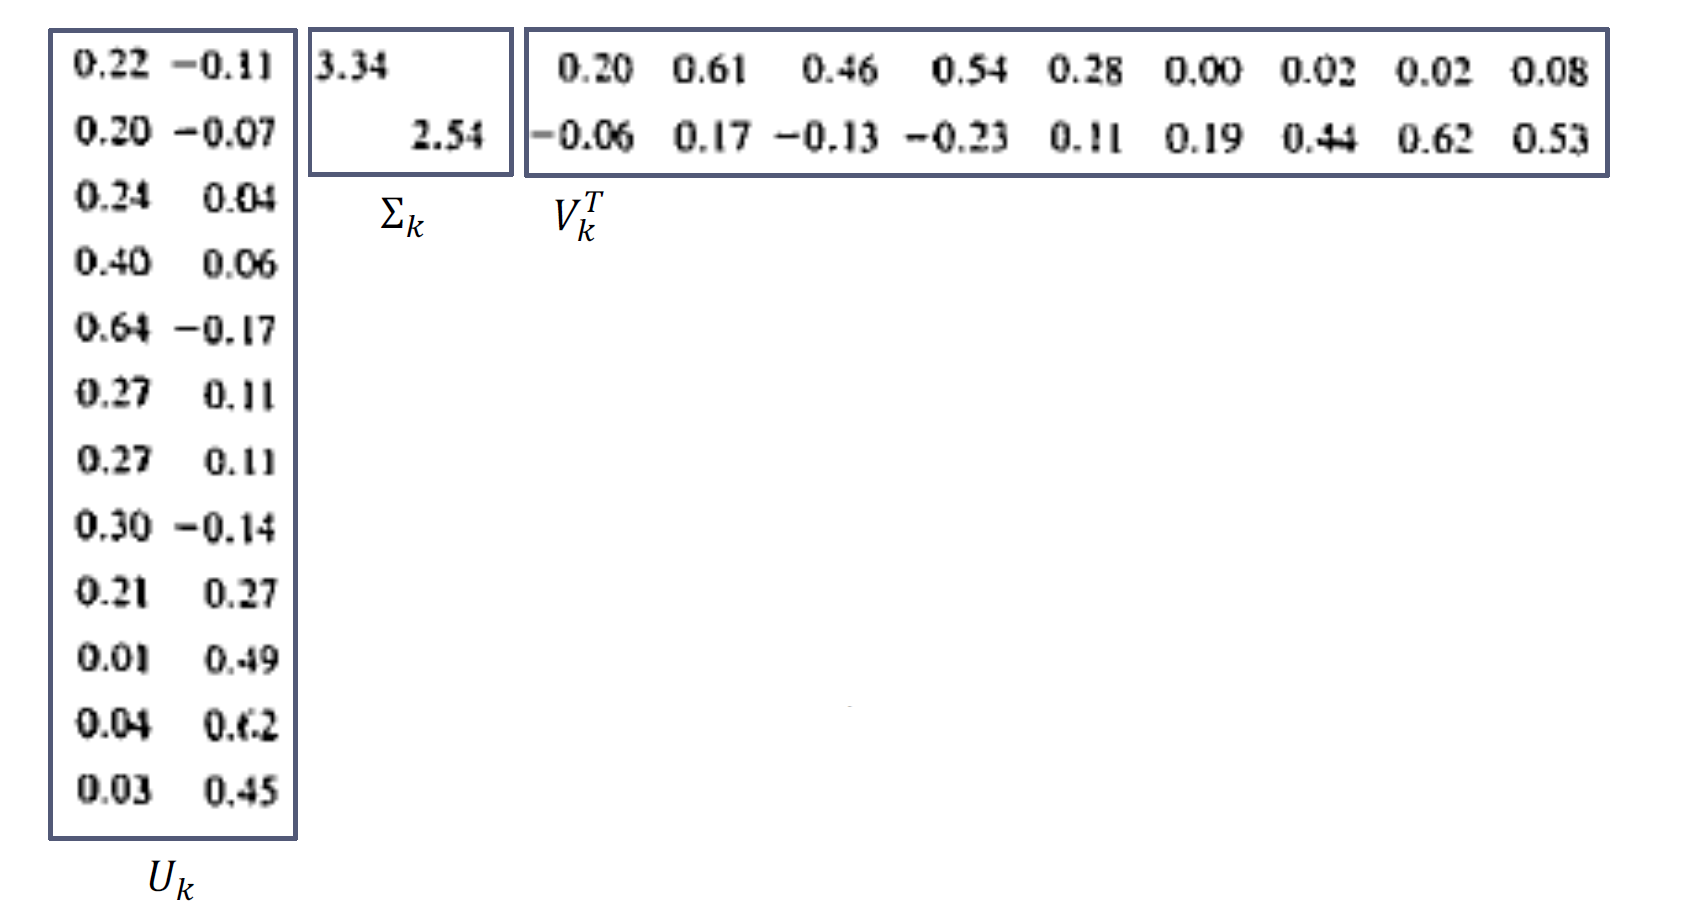
\includegraphics[width=\textwidth]{pic/7.png}
    \end{minipage}%
    \begin{minipage}{0.48\textwidth}
        \centering
        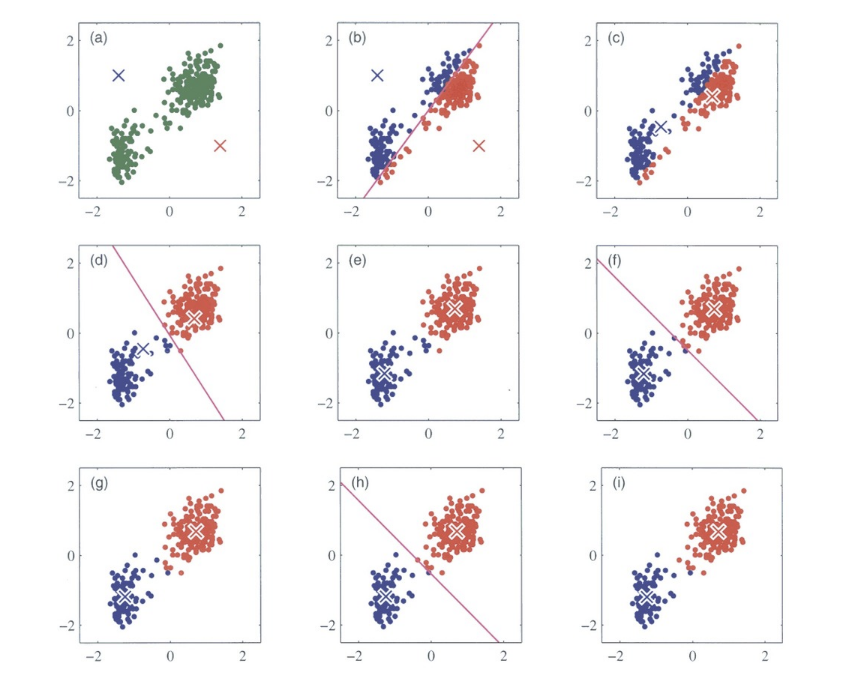
\includegraphics[width=\textwidth]{pic/8.png}
    \end{minipage}
    \vfill
    \begin{tikzpicture}[remember picture,overlay]
        \node[anchor=south west, xshift=0.1cm, yshift=0.22cm] at (current page.south west) {
            \scriptsize Figures adapted from slides of Andrew Ng, Machine Learning course, Stanford.
        };
    \end{tikzpicture}

\end{frame}

\begin{frame}{Cost function optimization}
    \begin{itemize}
        \item Weight update rule having $h_w(\mathbf{x}) = \mathbf{w}^T \mathbf{x}$ is as follows:
    \end{itemize}

    \[
    \mathbf{w}^{t+1} = \mathbf{w}^t + \eta \sum_{i=1}^{n} \left( y^{(i)} - \mathbf{w}^T \mathbf{x}^{(i)} \right) \mathbf{x}^{(i)}
    \]

    \begin{itemize}
        \item $\eta$: too small $\Rightarrow$ gradient descent can be slow.
        \item $\eta$: too large $\Rightarrow$ gradient descent can overshoot the minimum. It may fail to converge, or even diverge.
    \end{itemize}
\end{frame}

\begin{frame}{Gradient descent overview}
    \begin{minipage}{0.5\textwidth}
        \centering
        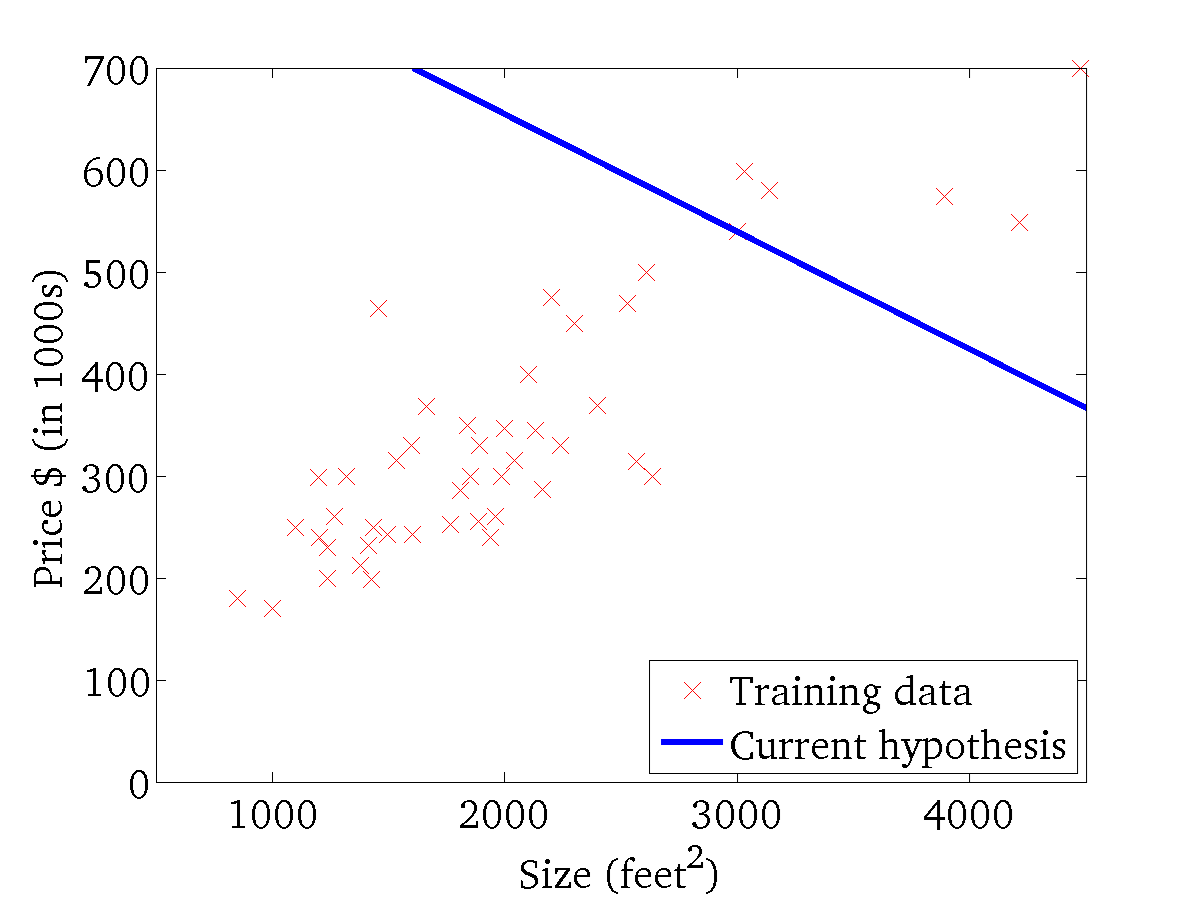
\includegraphics[width=1.0\textwidth]{pic/GD/hypothesis_1.png}
    \end{minipage}%
    \begin{minipage}{0.5\textwidth}
        \centering
        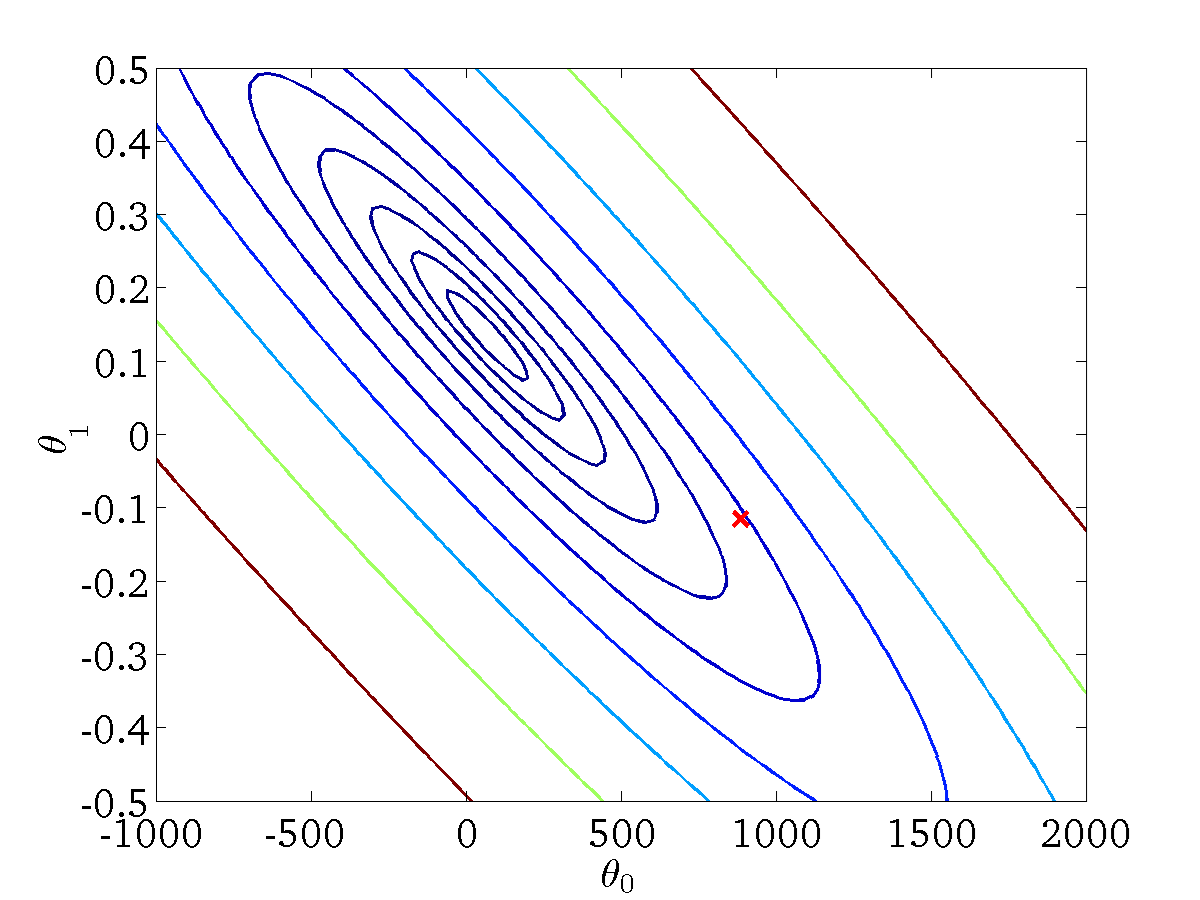
\includegraphics[width=1.0\textwidth]{pic/GD/cost_function_1.png}
    \end{minipage}
    \vfill
    \vfill
    \begin{tikzpicture}[remember picture,overlay]
        \node[anchor=south west, xshift=0.1cm, yshift=0.22cm] at (current page.south west) {
            \scriptsize Figures adapted from slides of Andrew Ng, Machine Learning course, Stanford.
        };
    \end{tikzpicture}
\end{frame}



\begin{frame}{Gradient descent overview (cont.)}
    \begin{minipage}{0.5\textwidth}
        \centering
        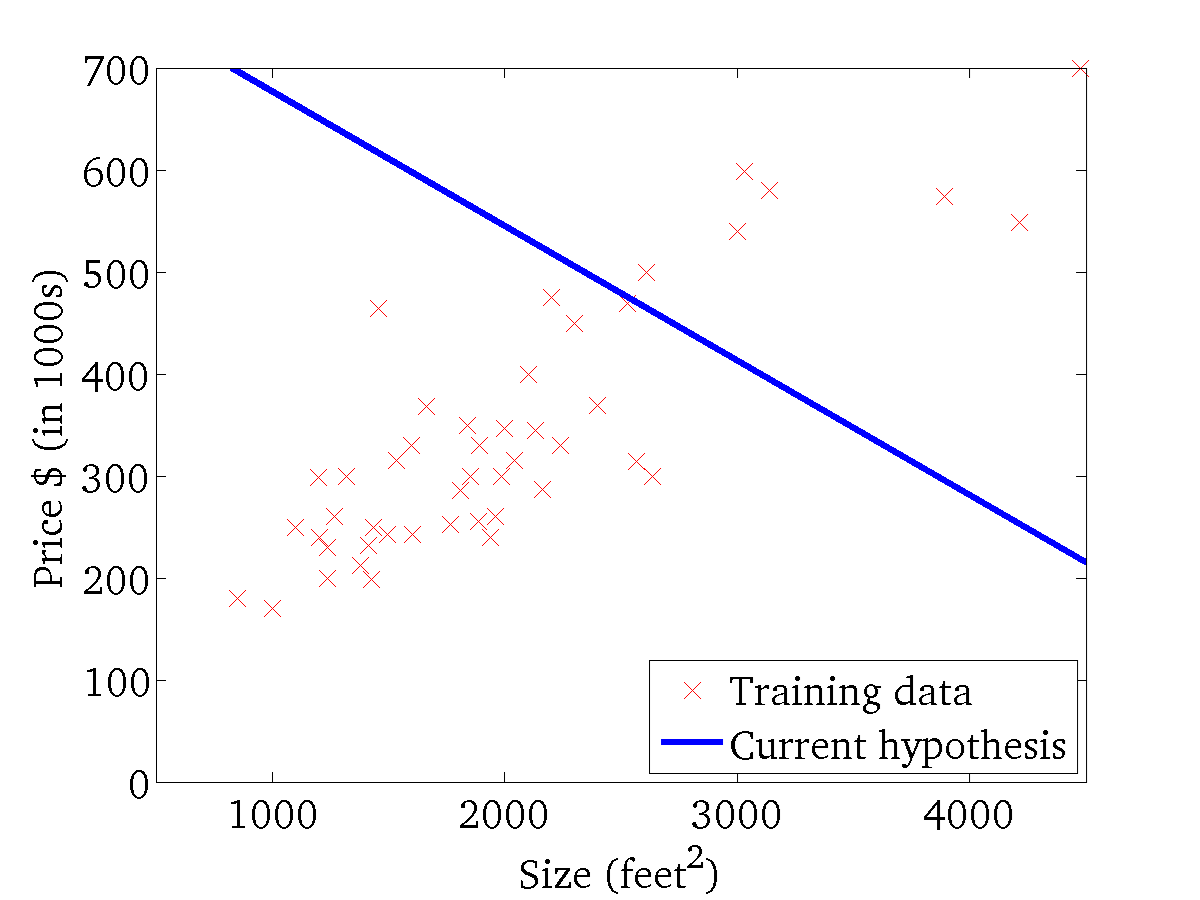
\includegraphics[width=1.0\textwidth]{pic/GD/hypothesis_2.png}
    \end{minipage}%
    \begin{minipage}{0.5\textwidth}
        \centering
        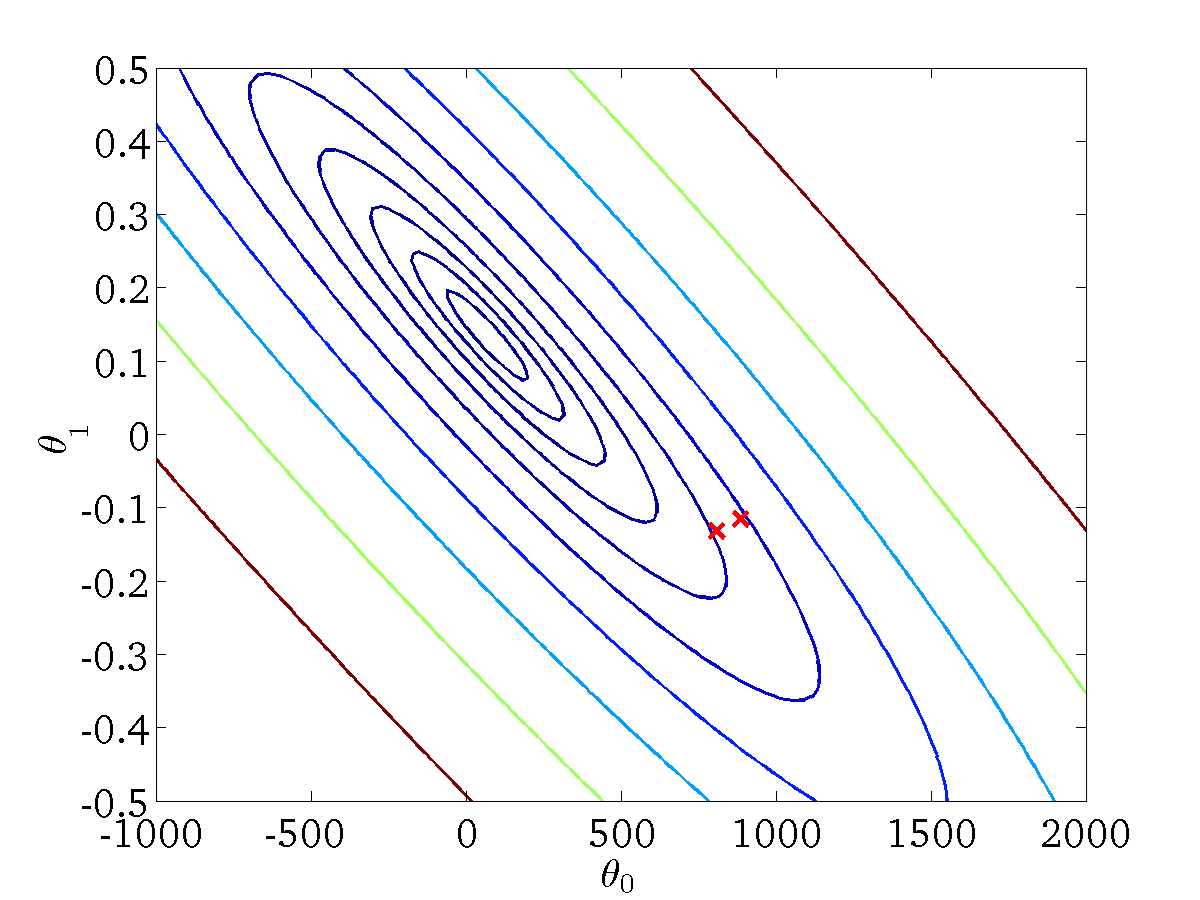
\includegraphics[width=1.0\textwidth]{pic/GD/cost_function_2.png}
    \end{minipage}
    \vfill
    \vfill
    \begin{tikzpicture}[remember picture,overlay]
        \node[anchor=south west, xshift=0.1cm, yshift=0.22cm] at (current page.south west) {
            \scriptsize Figures adapted from slides of Andrew Ng, Machine Learning course, Stanford.
        };
    \end{tikzpicture}
\end{frame}

\begin{frame}{Gradient descent overview (cont.)}
    \begin{minipage}{0.5\textwidth}
        \centering
        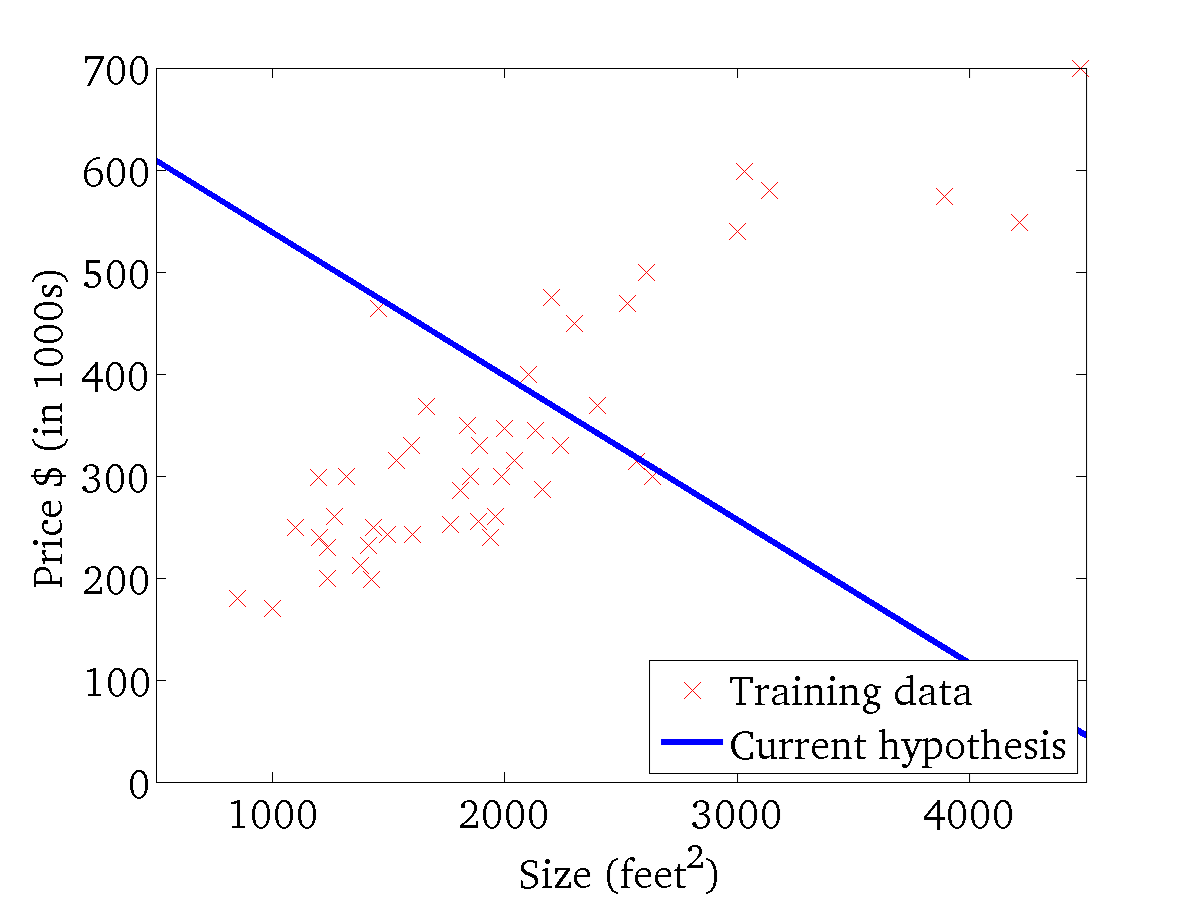
\includegraphics[width=1.0\textwidth]{pic/GD/hypothesis_3.png}
    \end{minipage}%
    \begin{minipage}{0.5\textwidth}
        \centering
        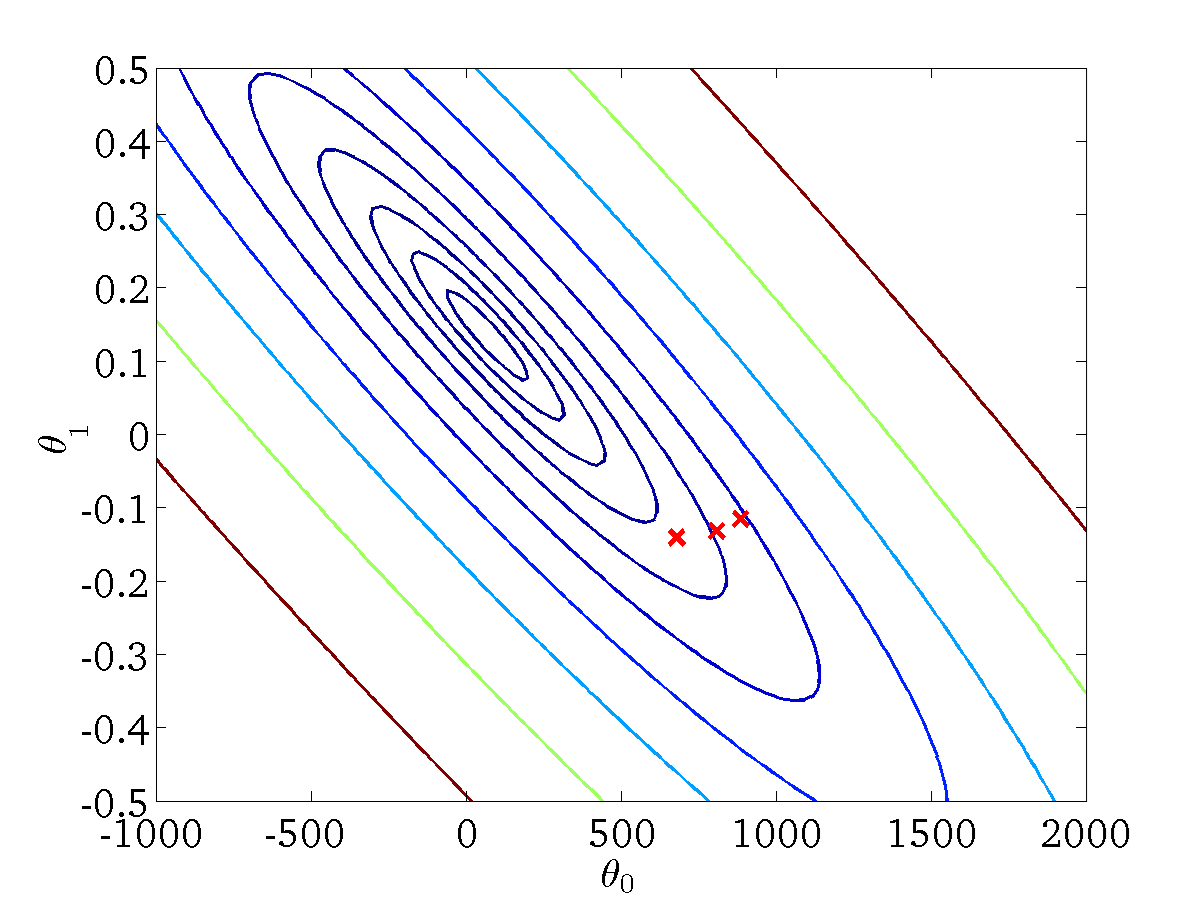
\includegraphics[width=1.0\textwidth]{pic/GD/cost_function_3.png}
    \end{minipage}
    \vfill
    \vfill
    \begin{tikzpicture}[remember picture,overlay]
        \node[anchor=south west, xshift=0.1cm, yshift=0.22cm] at (current page.south west) {
            \scriptsize Figures adapted from slides of Andrew Ng, Machine Learning course, Stanford.
        };
    \end{tikzpicture}
\end{frame}

\begin{frame}{Gradient descent overview (cont.)}
    \begin{minipage}{0.5\textwidth}
        \centering
        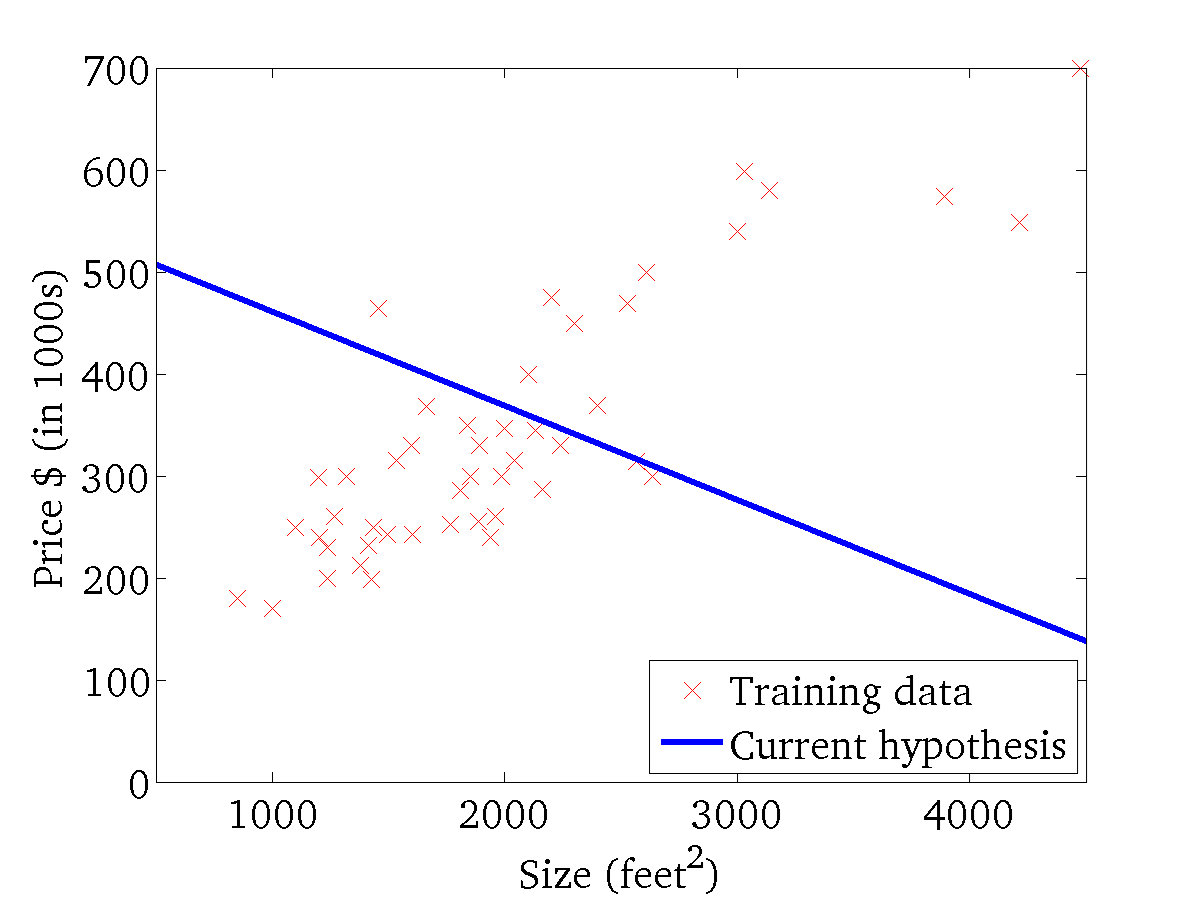
\includegraphics[width=1.0\textwidth]{pic/GD/hypothesis_4.png}
    \end{minipage}%
    \begin{minipage}{0.5\textwidth}
        \centering
        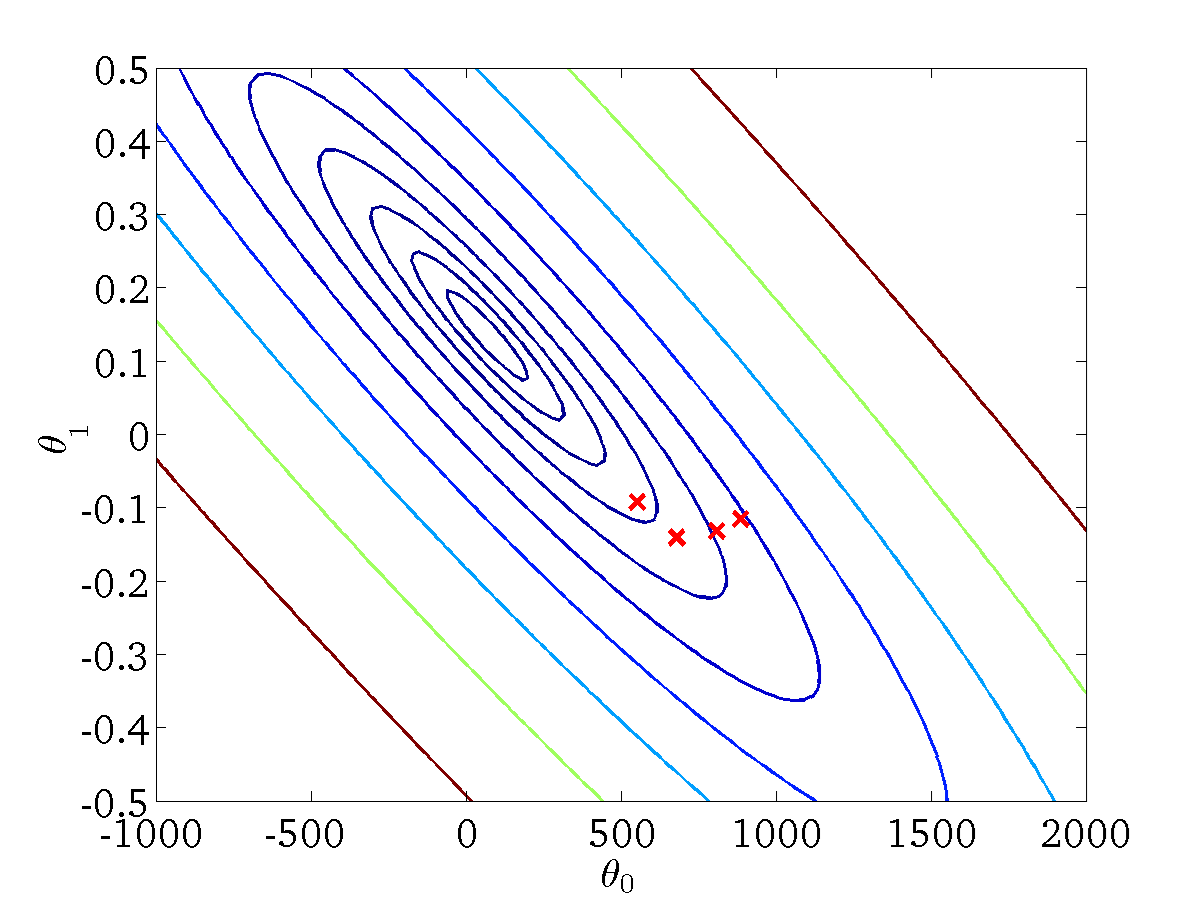
\includegraphics[width=1.0\textwidth]{pic/GD/cost_function_4.png}
    \end{minipage}
    \vfill
    \vfill
    \begin{tikzpicture}[remember picture,overlay]
        \node[anchor=south west, xshift=0.1cm, yshift=0.22cm] at (current page.south west) {
            \scriptsize Figures adapted from slides of Andrew Ng, Machine Learning course, Stanford.
        };
    \end{tikzpicture}
\end{frame}

\begin{frame}{Gradient descent overview (cont.)}
    \begin{minipage}{0.5\textwidth}
        \centering
        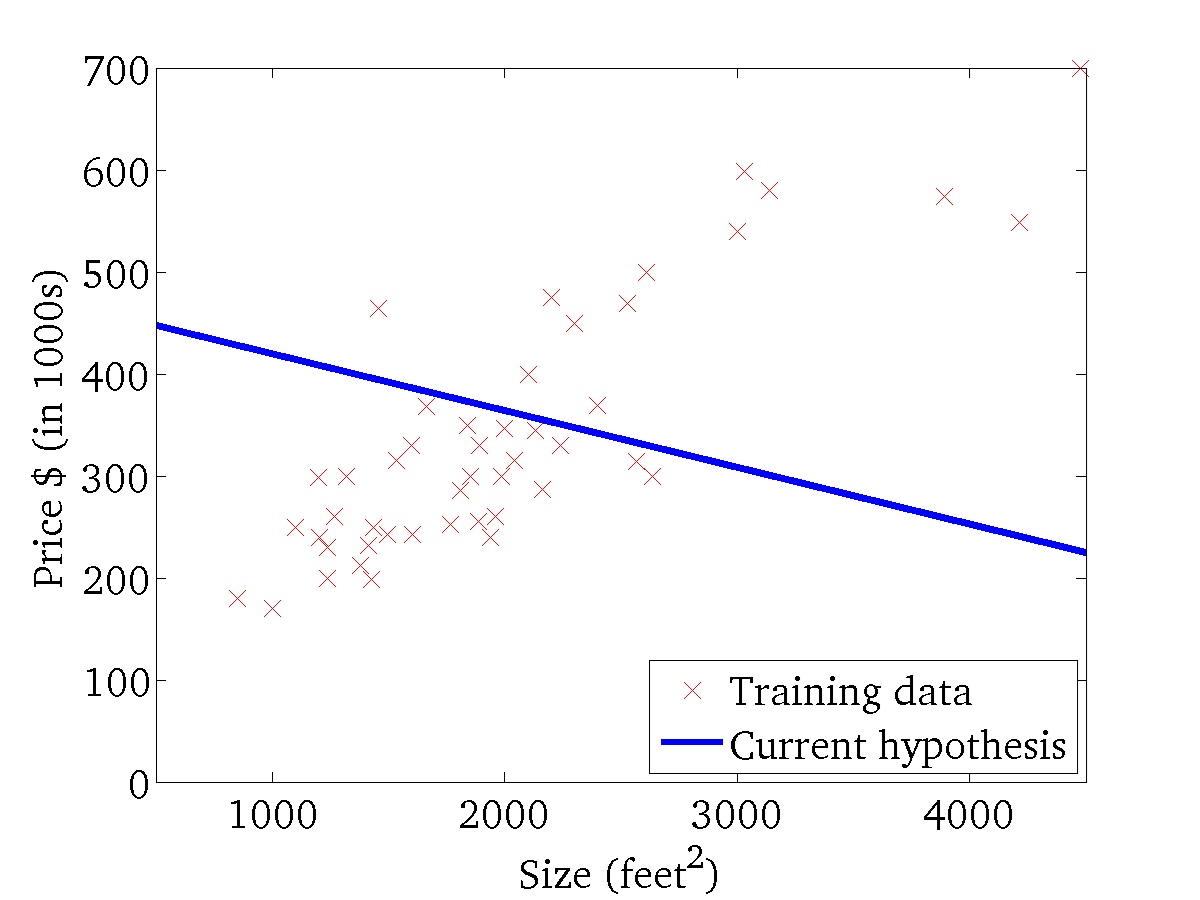
\includegraphics[width=1.0\textwidth]{pic/GD/hypothesis_5.png}
    \end{minipage}%
    \begin{minipage}{0.5\textwidth}
        \centering
        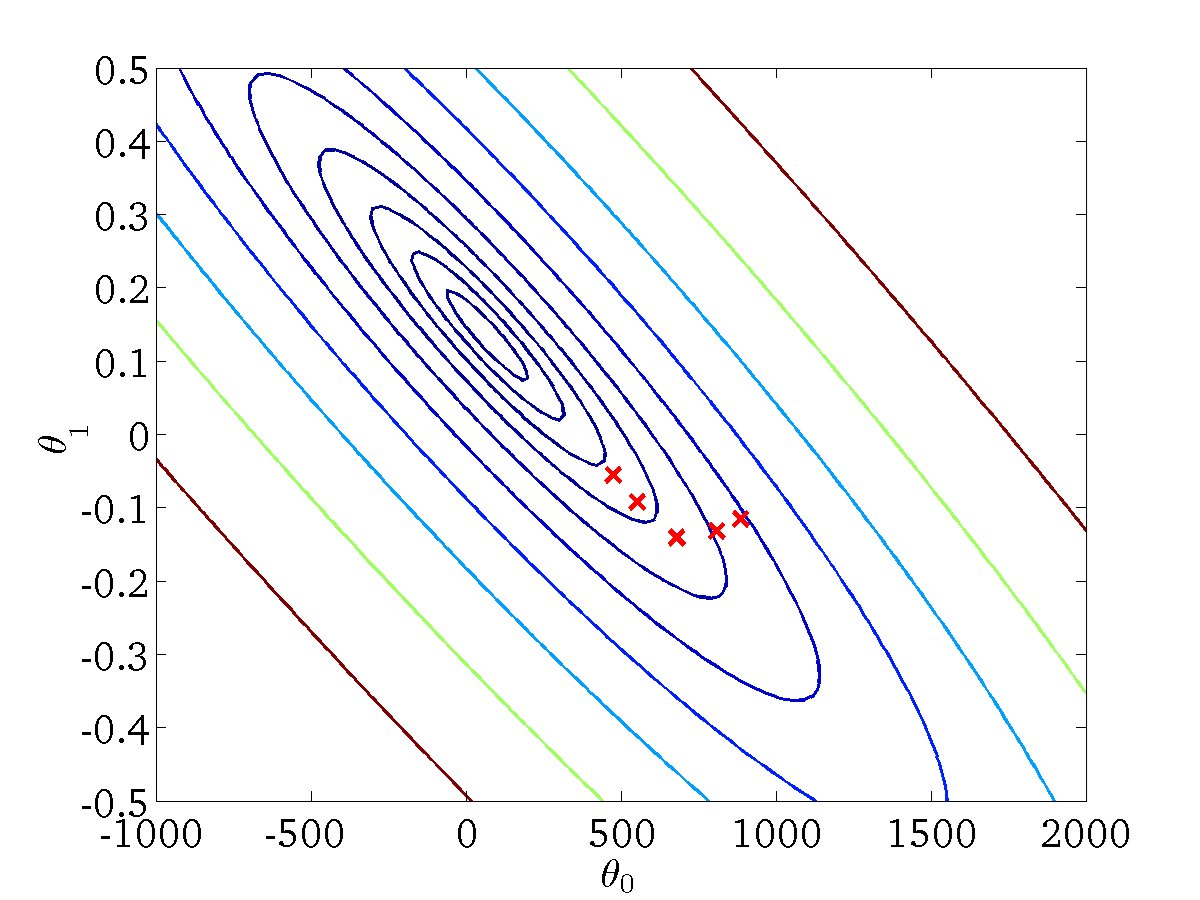
\includegraphics[width=1.0\textwidth]{pic/GD/cost_function_5.png}
    \end{minipage}
    \vfill
    \vfill
    \begin{tikzpicture}[remember picture,overlay]
        \node[anchor=south west, xshift=0.1cm, yshift=0.22cm] at (current page.south west) {
            \scriptsize Figures adapted from slides of Andrew Ng, Machine Learning course, Stanford.
        };
    \end{tikzpicture}
\end{frame}

\begin{frame}{Gradient descent overview (cont.)}
    \begin{minipage}{0.5\textwidth}
        \centering
        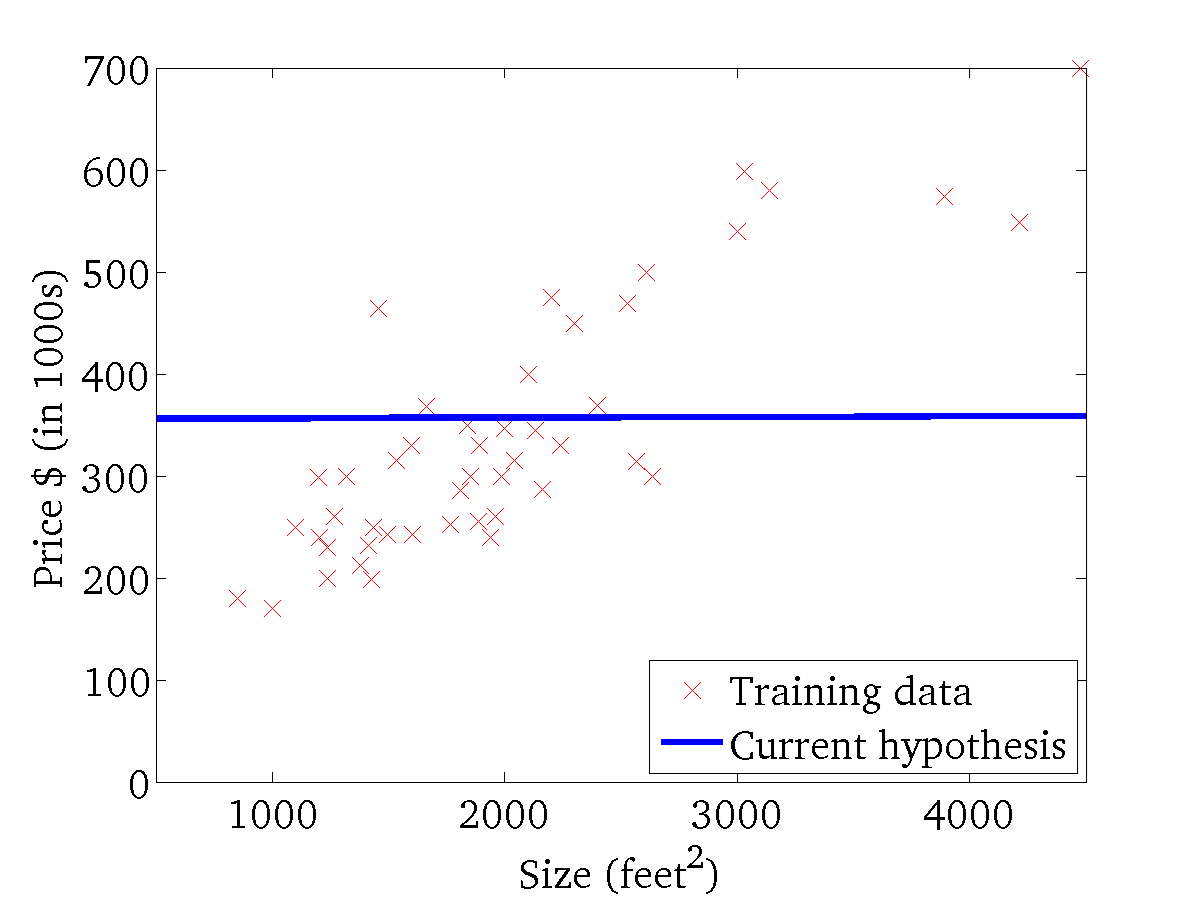
\includegraphics[width=1.0\textwidth]{pic/GD/hypothesis_6.png}
    \end{minipage}%
    \begin{minipage}{0.5\textwidth}
        \centering
        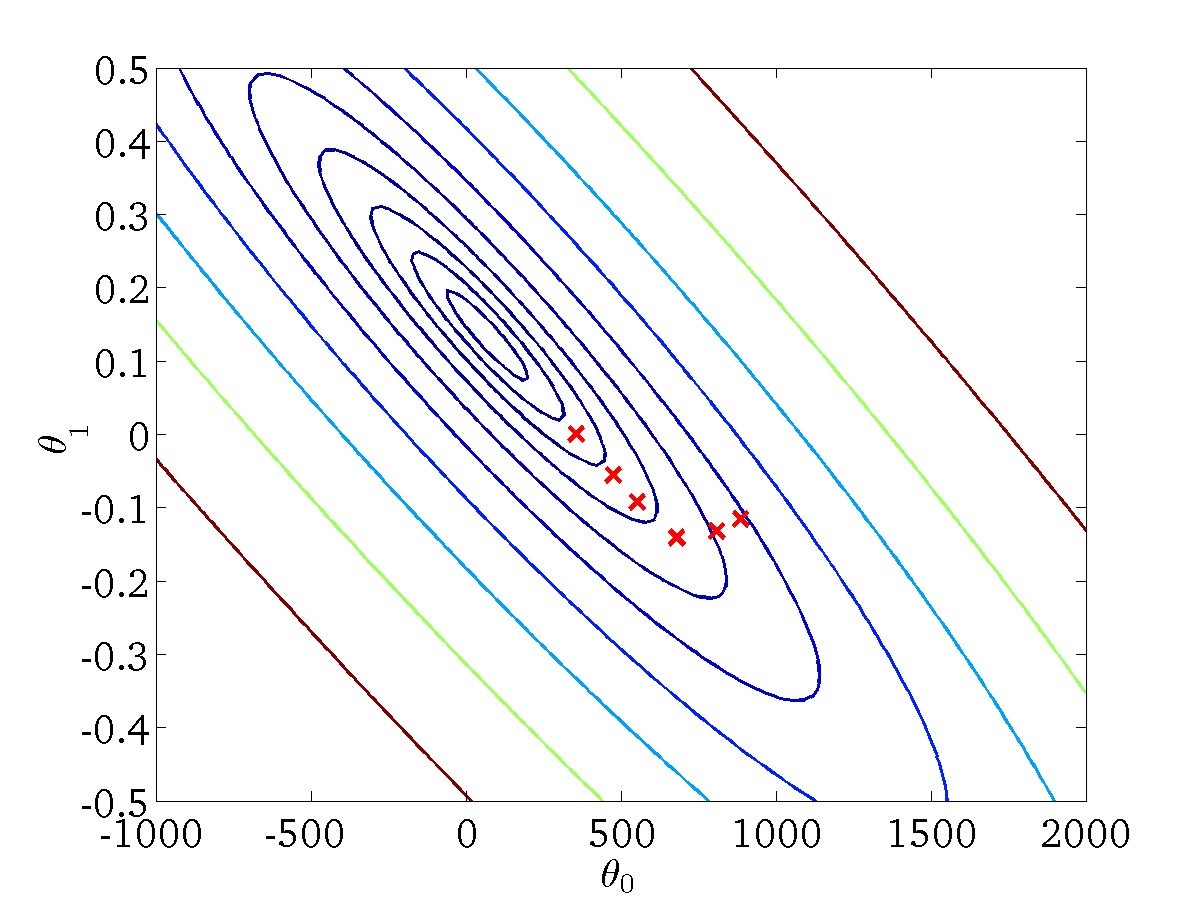
\includegraphics[width=1.0\textwidth]{pic/GD/cost_function_6.png}
    \end{minipage}
    \vfill
    \vfill
    \begin{tikzpicture}[remember picture,overlay]
        \node[anchor=south west, xshift=0.1cm, yshift=0.22cm] at (current page.south west) {
            \scriptsize Figures adapted from slides of Andrew Ng, Machine Learning course, Stanford.
        };
    \end{tikzpicture}
\end{frame}

\begin{frame}{Gradient descent overview (cont.)}
    \begin{minipage}{0.5\textwidth}
        \centering
        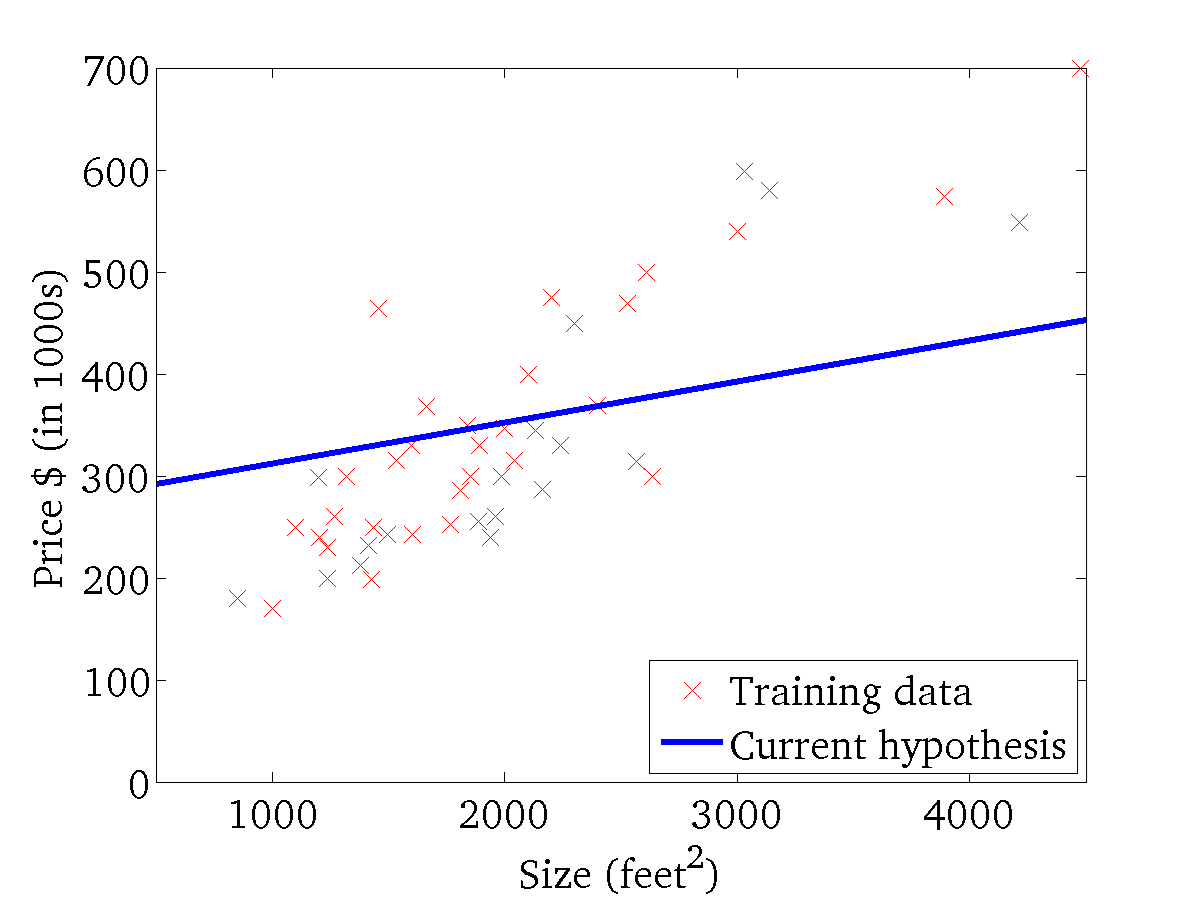
\includegraphics[width=1.0\textwidth]{pic/GD/hypothesis_7.png}
    \end{minipage}%
    \begin{minipage}{0.5\textwidth}
        \centering
        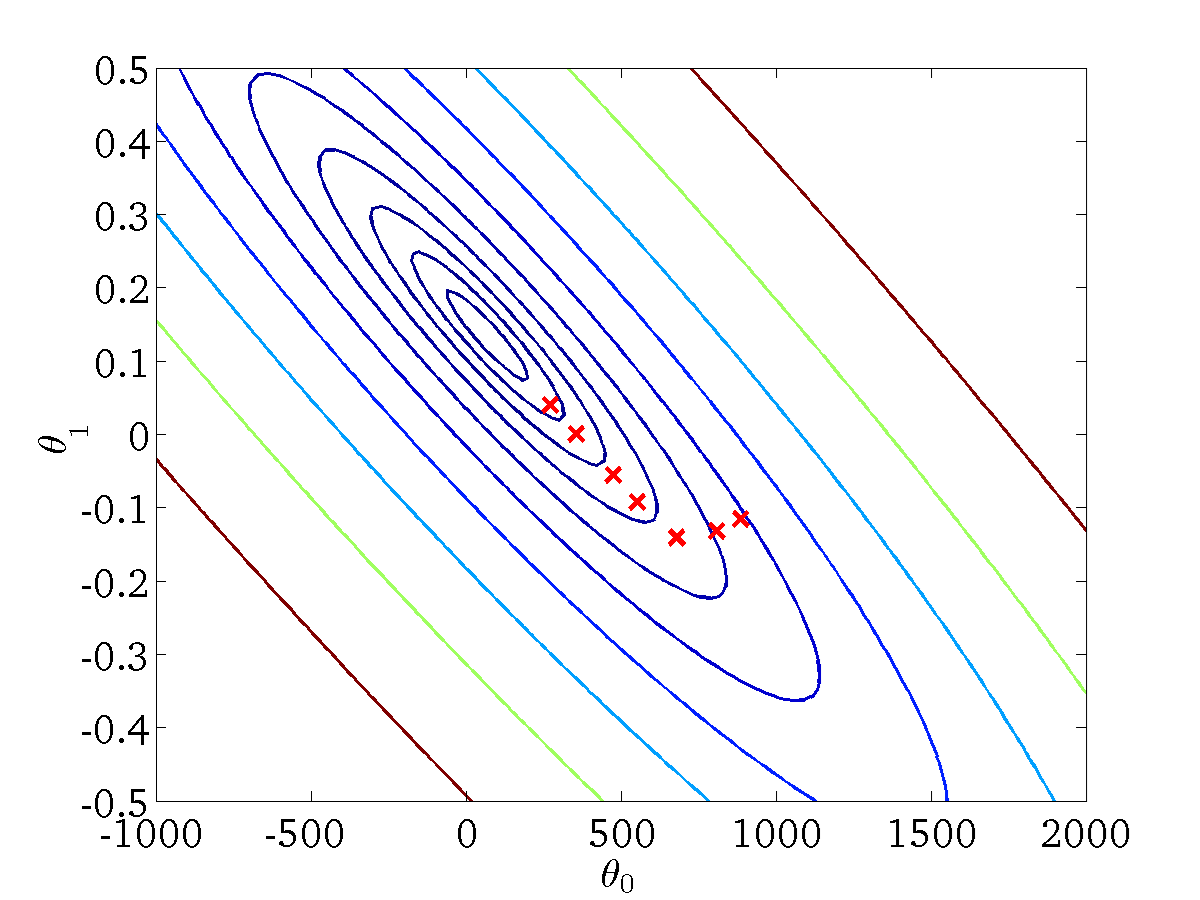
\includegraphics[width=1.0\textwidth]{pic/GD/cost_function_7.png}
    \end{minipage}
    \vfill
    \vfill
    \begin{tikzpicture}[remember picture,overlay]
        \node[anchor=south west, xshift=0.1cm, yshift=0.22cm] at (current page.south west) {
            \scriptsize Figures adapted from slides of Andrew Ng, Machine Learning course, Stanford.
        };
    \end{tikzpicture}
\end{frame}

\begin{frame}{Gradient descent overview (cont.)}
    \begin{minipage}{0.5\textwidth}
        \centering
        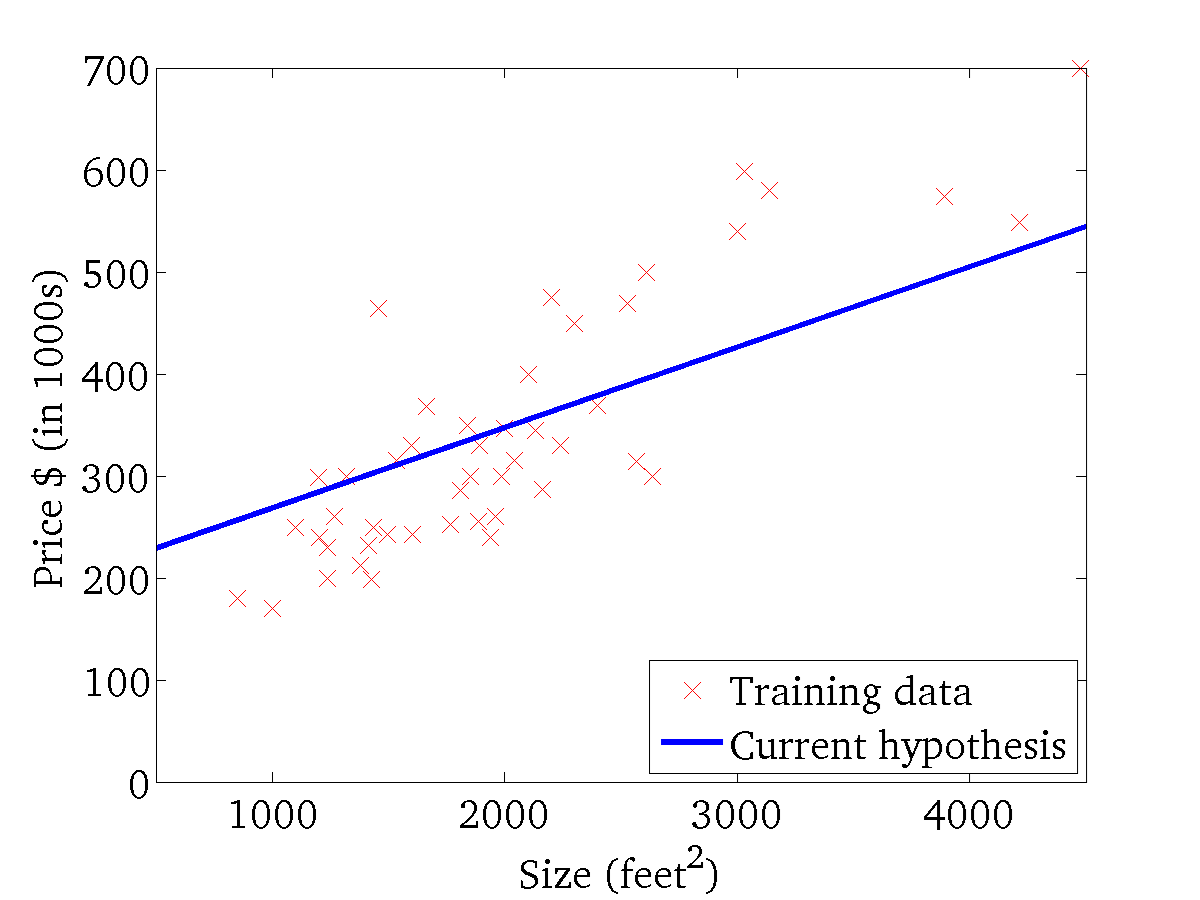
\includegraphics[width=1.0\textwidth]{pic/GD/hypothesis_8.png}
    \end{minipage}%
    \begin{minipage}{0.5\textwidth}
        \centering
        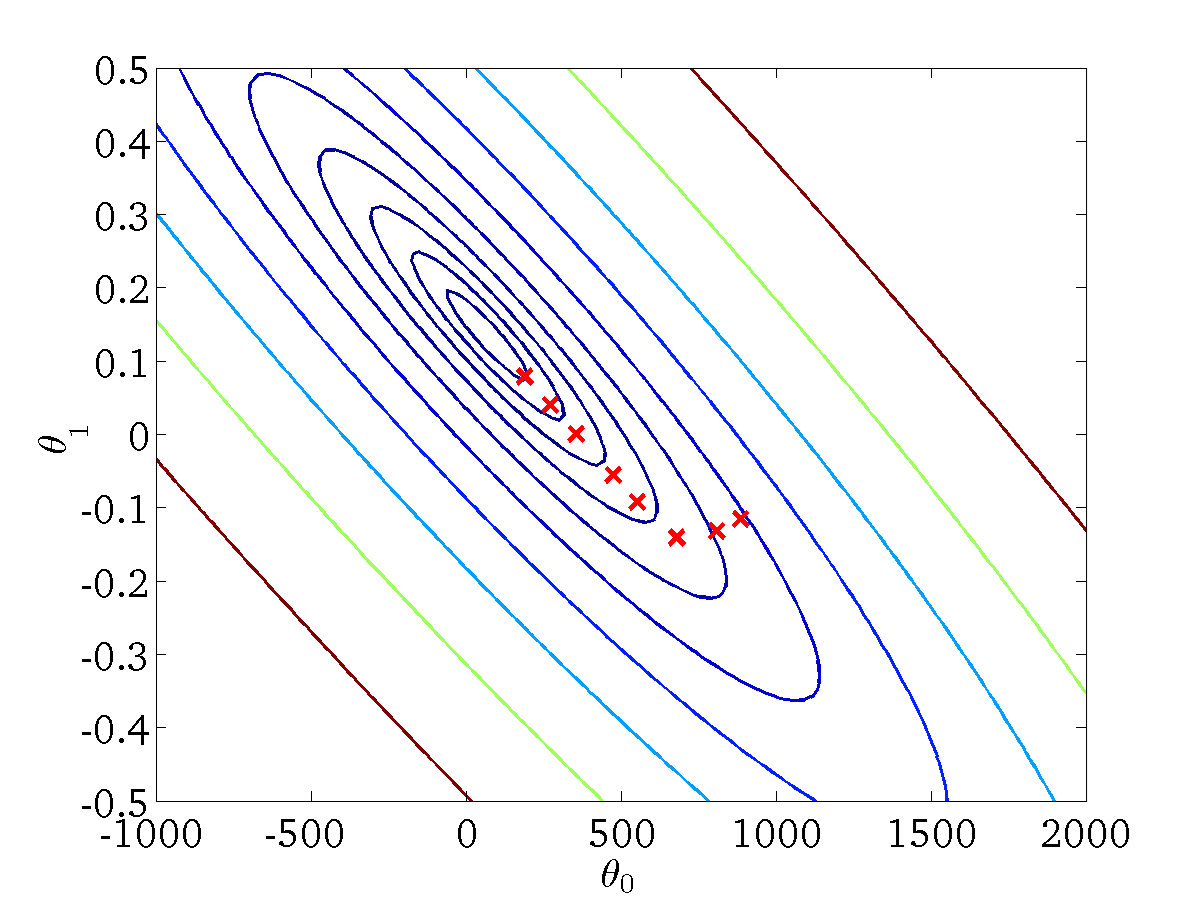
\includegraphics[width=1.0\textwidth]{pic/GD/cost_function_8.png}
    \end{minipage}
    \vfill
    \vfill
    \begin{tikzpicture}[remember picture,overlay]
        \node[anchor=south west, xshift=0.1cm, yshift=0.22cm] at (current page.south west) {
            \scriptsize Figures adapted from slides of Andrew Ng, Machine Learning course, Stanford.
        };
    \end{tikzpicture}
\end{frame}

\begin{frame}{Gradient descent overview (cont.)}
    \begin{minipage}{0.5\textwidth}
        \centering
        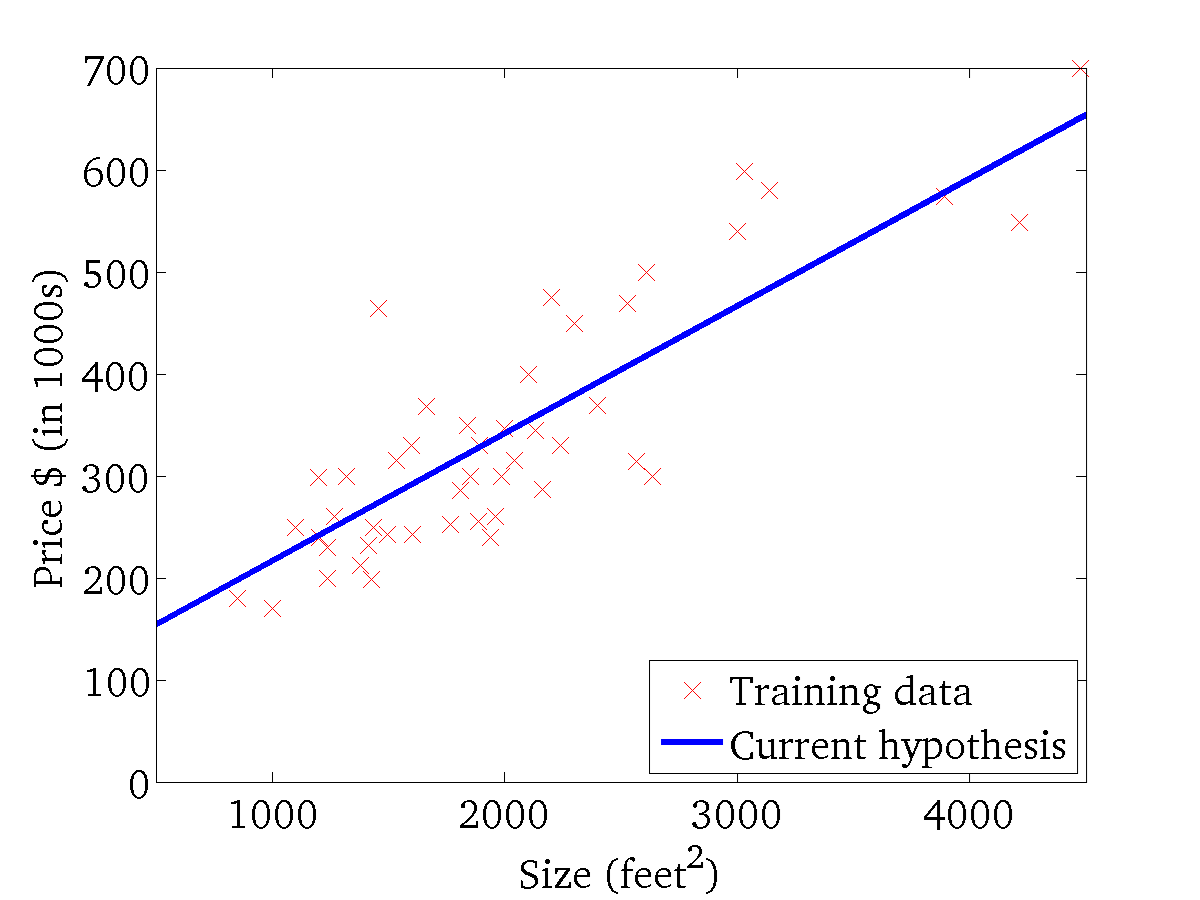
\includegraphics[width=1.0\textwidth]{pic/GD/hypothesis_9.png}
    \end{minipage}%
    \begin{minipage}{0.5\textwidth}
        \centering
        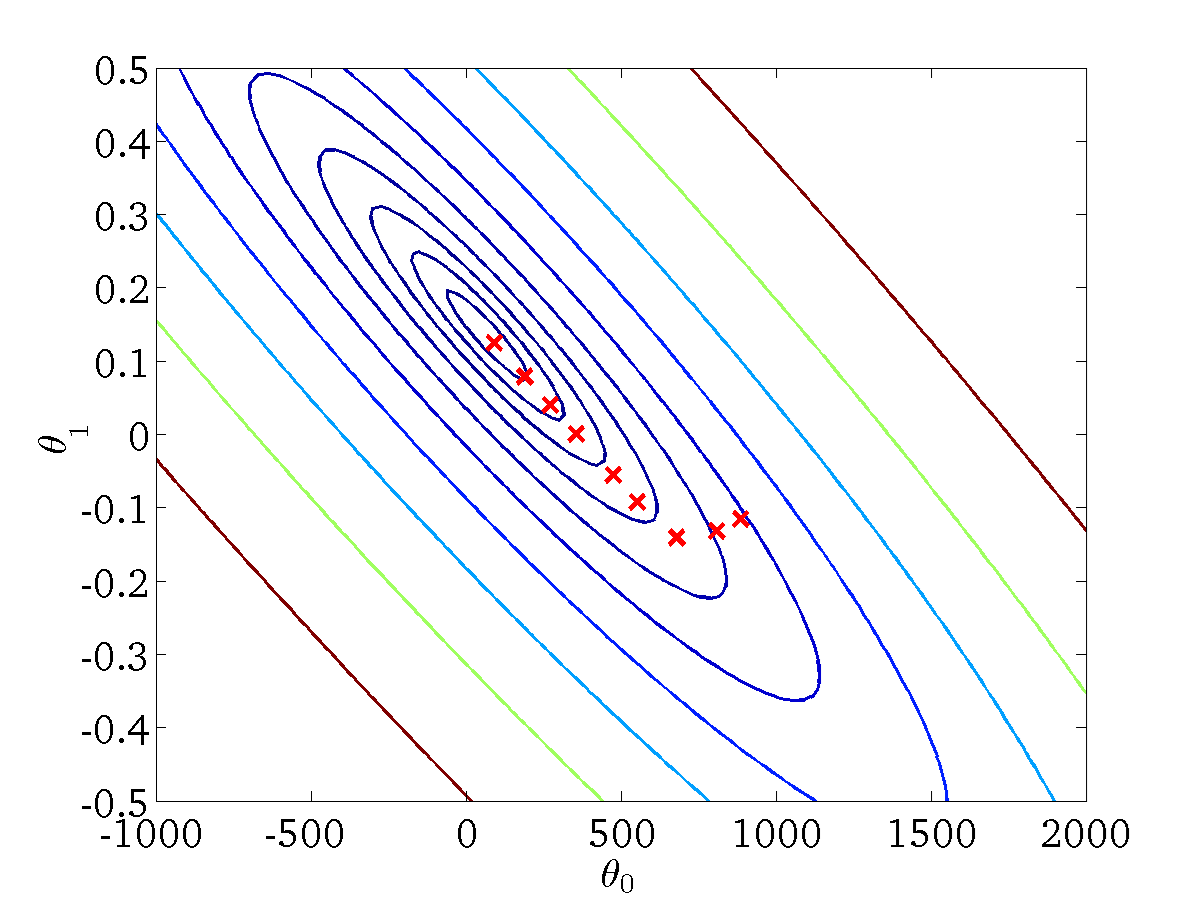
\includegraphics[width=1.0\textwidth]{pic/GD/cost_function_9.png}
    \end{minipage}
    \vfill
    \vfill
    \begin{tikzpicture}[remember picture,overlay]
        \node[anchor=south west, xshift=0.1cm, yshift=0.22cm] at (current page.south west) {
            \scriptsize Figures adapted from slides of Andrew Ng, Machine Learning course, Stanford.
        };
    \end{tikzpicture}
\end{frame}




\begin{frame}{Variants of gradient descent}
    \begin{itemize}
        \item \textbf{Batch gradient descent:} processes the entire training set in one iteration
        \begin{itemize}
            \item It can be computationally costly for large data sets and practically impossible for some applications (such as online learning).
        \end{itemize}

        \item \textbf{Mini-batch gradient descent:} processes small, random subsets (mini-batches) of the training set in each iteration
        \begin{itemize}
            \item Balances the efficiency of batch gradient descent.
            % \item Reduces variance in the parameter updates, leading to more stable convergence.
        \end{itemize}
        \item \textbf{Stochastic gradient descent:} processes one training example per iteration
        \begin{itemize}
            \item Updates the model parameters more frequently, which can lead to faster convergence.
            % \item Introduces noise into the optimization process, which can help escape local minima.
            % \item Can be less stable and more sensitive to the learning rate.
        \end{itemize}
    \end{itemize}
        % \[
    % J(\mathbf{w}) = \sum_{i=1}^{n} J^{(i)}(\mathbf{w})
    % \]

    % \begin{itemize}
    %     \item \textbf{Update after presentation of} $(\mathbf{x}^{(i)}, y^{(i)})$:
    % \end{itemize}

    % \[
    % \mathbf{w}^{t+1} = \mathbf{w}^t - \eta \nabla_{\mathbf{w}} J^{(i)}(\mathbf{w})
    % \]
\end{frame}

\begin{frame}{Stochastic gradient descent}

    \begin{itemize}
        \item \textbf{Example:} Linear regression with SSE cost function
    \end{itemize}
    \[
    J(\mathbf{w}) = \sum_{i=1}^{n} J^{(i)}(\mathbf{w})
    \]

    \[
    J^{(i)}(\mathbf{w}) = \left( y^{(i)} - \mathbf{w}^T \mathbf{x}^{(i)} \right)^2
    \]

    \[
    \mathbf{w}^{t+1} = \mathbf{w}^t - \eta \nabla_{\mathbf{w}} J^{(i)}(\mathbf{w})
    \]

    \[
    \implies \mathbf{w}^{t+1} = \mathbf{w}^t + \eta \left( y^{(i)} - \mathbf{w}^T \mathbf{x}^{(i)} \right) \mathbf{x}^{(i)}
    \]

    \begin{center}
        In which \( x^{(i)} \) indicates the \(i\)'th observation arrived.
    \end{center}

\end{frame}


% \begin{frame}{Stochastic gradient descent: online learning}
%     \begin{itemize}
%         \item \textbf{Online learning} is also appropriate for real-time applications
%         \begin{itemize}
%             \item Data observations are arriving in a continuous stream
%             \item Predictions must be made before seeing all of the data
%         \end{itemize}
%     \end{itemize}
% \end{frame}

\begin{frame}{Stochastic gradient descent: online learning}

    \begin{itemize}
        \item Often, stochastic gradient descent gets close to the minimum much faster than batch gradient descent.
        \item Note however that it may never converge to the minimum, and the parameters will keep oscillating around the minimum of the cost function;
        \begin{itemize}
            \item In practice, most of the values near the minimum will be reasonably good approximations to the true minimum.
        \end{itemize}
    \end{itemize}

\end{frame}


\begin{frame}{Newton's Method}
    \begin{itemize}
        \item Newton's method assumes that the loss $\ell$ is \textbf{twice differentiable}
        and uses the approximation with the Hessian (2nd order Taylor approximation).
        \item The \textbf{Hessian Matrix} contains all second-order partial derivatives and is defined as:
    \end{itemize}

    \[
    H(\mathbf{w}) =
    \begin{pmatrix}
        \frac{\partial^2 \ell}{\partial w_1^2} & \frac{\partial^2 \ell}{\partial w_1 \partial w_2} & \cdots & \frac{\partial^2 \ell}{\partial w_1 \partial w_n} \\
        \vdots & \ddots & & \vdots \\
        \frac{\partial^2 \ell}{\partial w_n \partial w_1} & \cdots & \cdots & \frac{\partial^2 \ell}{\partial w_n^2}
    \end{pmatrix}.
    \]

    \begin{itemize}
        \item Because of the convexity of $\ell$, it is a symmetric, positive semi-definite matrix.
        \item \textbf{Note:} A symmetric matrix $M$ is positive semi-definite if it has only non-negative eigenvalues, or equivalently,
        for any vector $\mathbf{x}$ we have $\mathbf{x}^{\top}M\mathbf{x} \ge 0$.
    \end{itemize}
\end{frame}


\begin{frame}{Newton's Method (cont.)}
    \begin{itemize}
        \item The second-order approximation of $\ell(\mathbf{w} + \mathbf{s})$ is:
        \[
        \ell(\mathbf{w} + \mathbf{s}) \approx \ell(\mathbf{w}) + g(\mathbf{w})^{\top} \mathbf{s} + \frac{1}{2}\mathbf{s}^{\top} H(\mathbf{w})\mathbf{s}.
        \]
        \item This describes a convex parabola, and we can find its minimum by solving:
        \[
        \arg\min_{\mathbf{s}} \, \ell(\mathbf{w}) + g(\mathbf{w})^{\top}\mathbf{s} + \frac{1}{2}\mathbf{s}^{\top} H(\mathbf{w})\mathbf{s}.
        \]
        \item Taking the derivative with respect to $\mathbf{s}$ and setting it to zero:
        \[
        g(\mathbf{w}) + H(\mathbf{w})\mathbf{s} = 0
        \quad \Rightarrow \quad
        \mathbf{s} = -[H(\mathbf{w})]^{-1} g(\mathbf{w}).
        \]
        \item Newton’s method converges extremely fast if the approximation is accurate
        and the step size is sufficiently small.
    \end{itemize}
\end{frame}


\begin{frame}{Newton's Method (cont.)}
\begin{itemize}
    \item Approximate the Hessian $H(\mathbf{w})$ with its diagonal to combine Newton's method and gradient descent, scaling steps by the inverse Hessian.
    \item Use gradient descent first, then switch to Newton's method near the optimum for stability and accuracy.
\end{itemize}
 \centering
    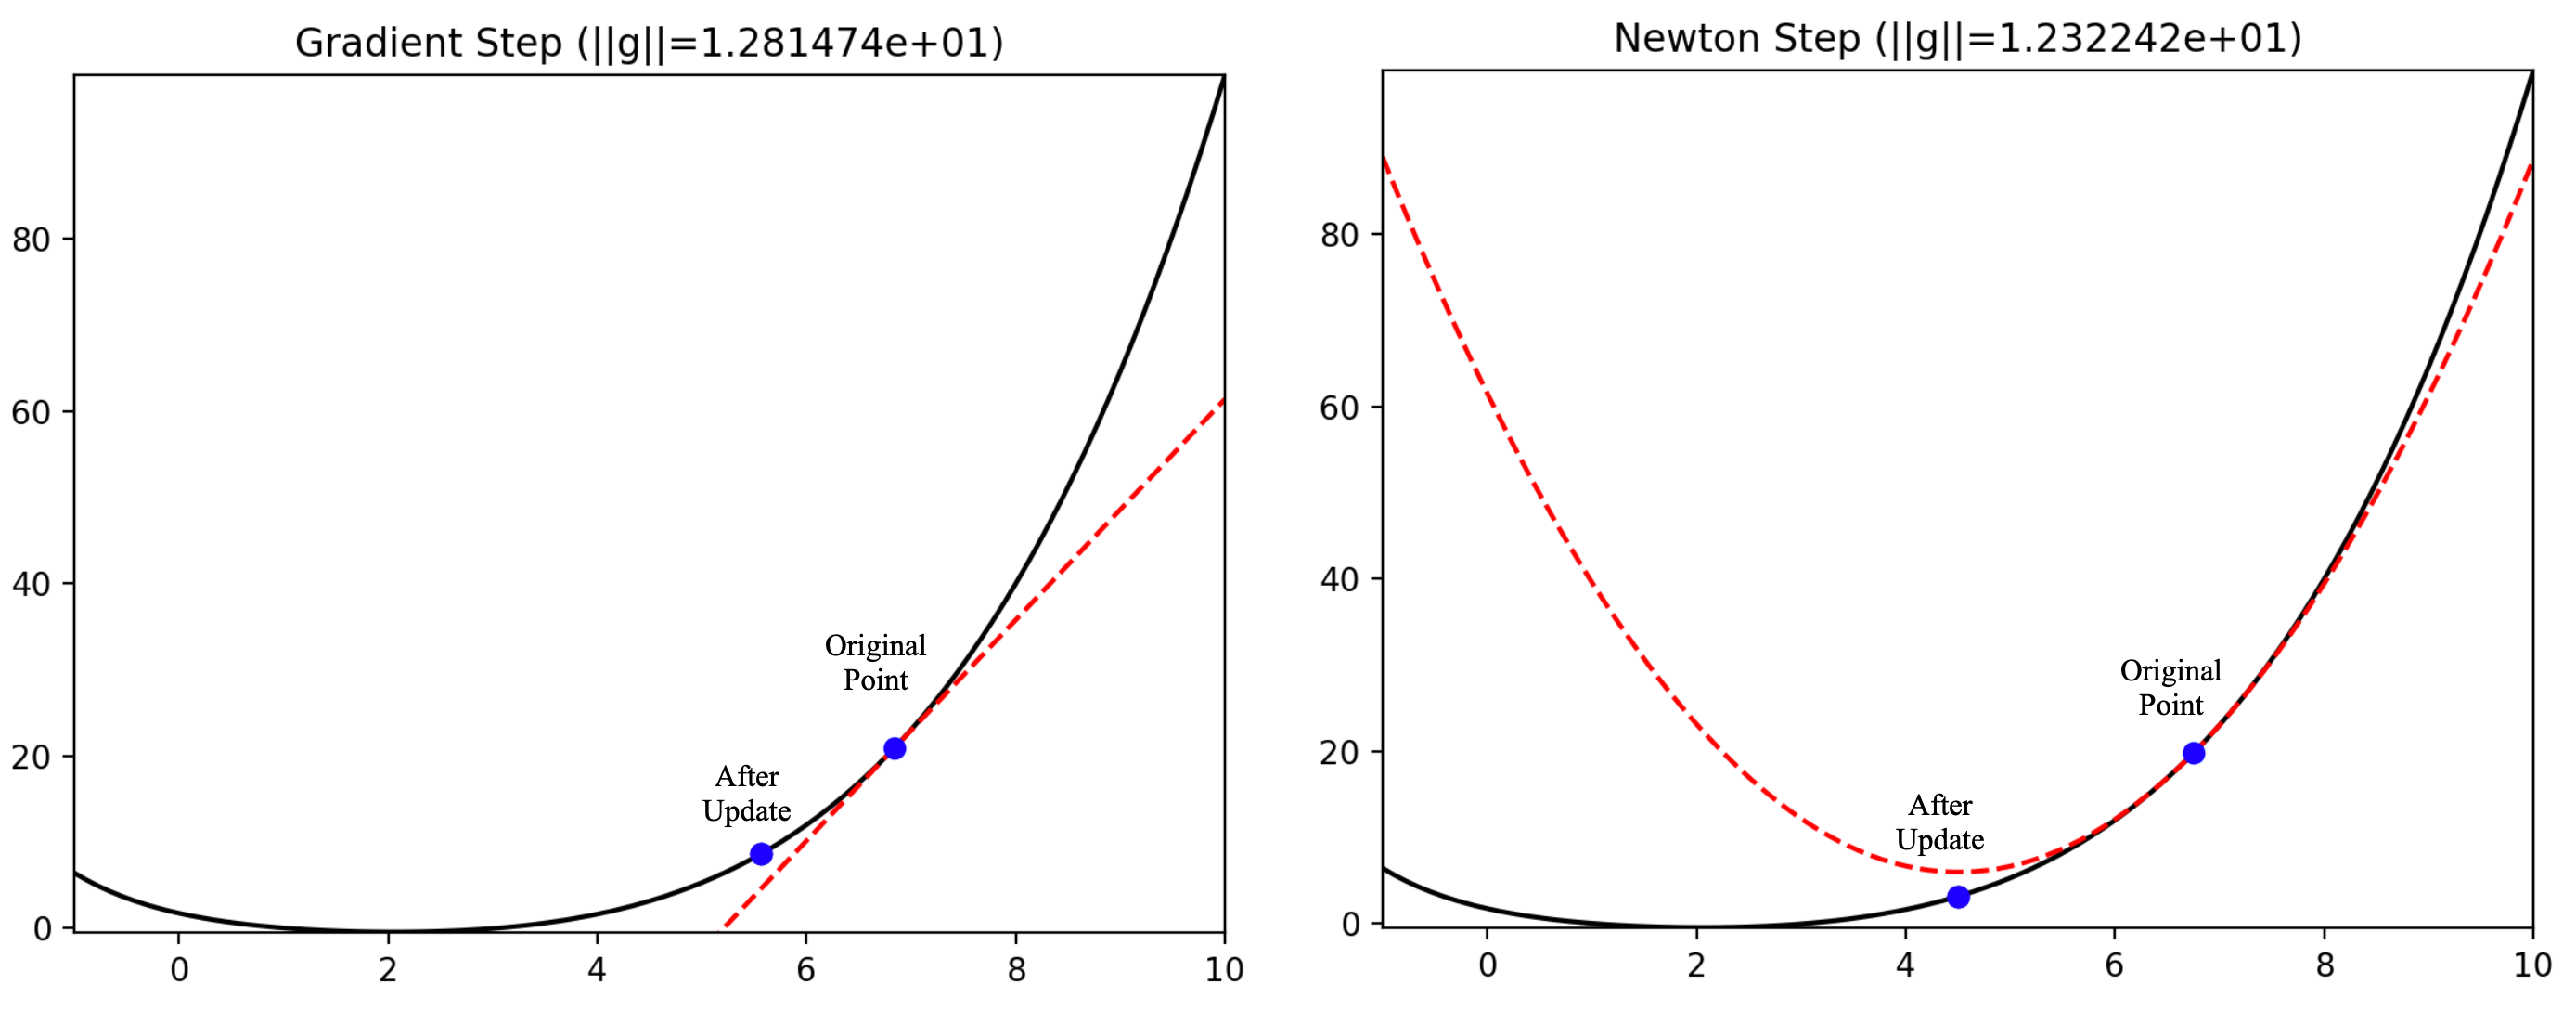
\includegraphics[width=0.7\linewidth]{pic/newton.png}
\end{frame}


\begin{frame}{Limitations of linear regression}
    \begin{itemize}
        \item It is possible that the best fitted line is still far off the real pattern of samples:
        \begin{figure}[h]
            \centering
            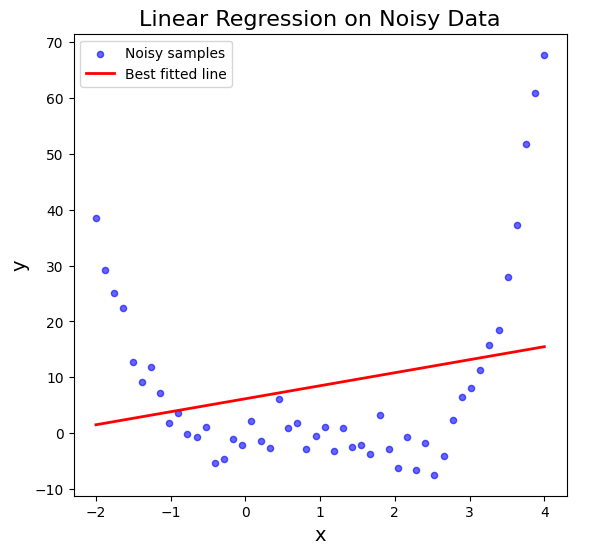
\includegraphics[width=0.45\textwidth]{pic/Polynomial_regression/best_fitted_line.png}
            \caption{No line can be fitted to generalize on these samples}
        \end{figure}
    \end{itemize}
\end{frame}


\begin{frame}{Beyond Linear Regression}
    \begin{itemize}
        \item How can we extend linear regression to model non-linear relationships?
        \begin{itemize}
            \item \textbf{Transforming Data Using Basis Functions:}
            \begin{itemize}
                \item Basis functions allow us to transform the original features into a new feature space.
                \item Common basis functions include polynomial and Gaussian functions.
            \end{itemize}
            \item \textbf{Learning a Linear Regression on Transformed Features:}
            \begin{itemize}
                \item By applying linear regression to the transformed feature vectors, we can model complex, non-linear relationships.
                \item This approach maintains the simplicity and interpretability of linear regression while extending its flexibility.
            \end{itemize}
        \end{itemize}
    \end{itemize}
\end{frame}

\begin{frame}{Beyond Linear Regression: Polynomial Regression}
    \begin{figure}[h]
        \centering
        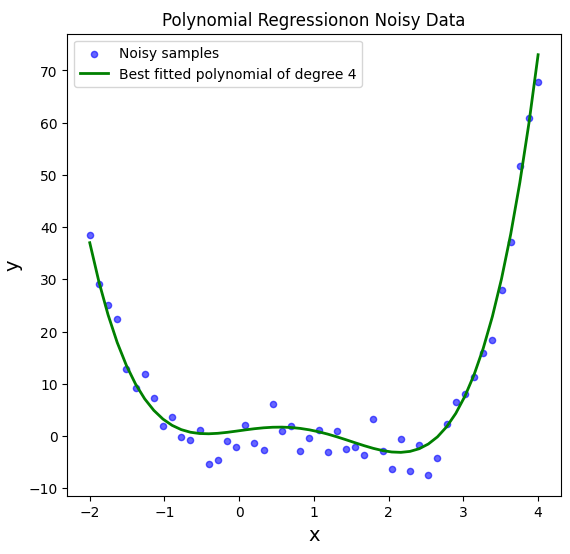
\includegraphics[width=0.45\textwidth]{pic/Polynomial_regression/best_fitted_polynomial.png}
        \caption{Best fitted polynomial of degree 4 can generalize well on samples}
    \end{figure}
\end{frame}


\begin{frame}{Beyond Linear Regression: change of basis}
    % \begin{minipage}
    \begin{figure}[h]
    \centering
    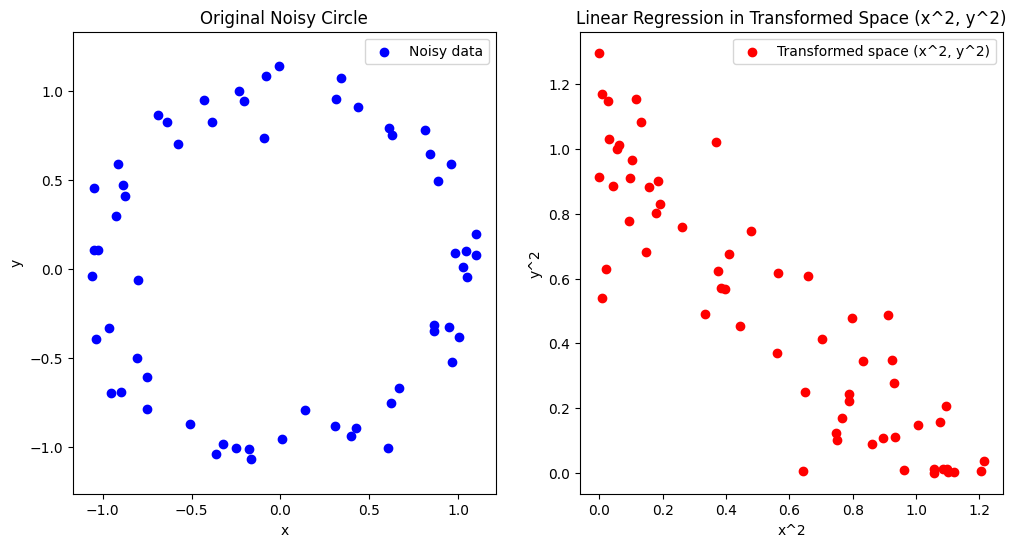
\includegraphics[width=0.75\textwidth]{pic/Polynomial_regression/change_of_basis.png}
    \caption{Changing the basis of \( [1, x, y] \) to \( [1, x^2, y^2] \), we can use linear regression}
    \end{figure}
    % \end{minipage}
\end{frame}

\begin{frame}{Polynomial regression: Univariate}
    \begin{itemize}
        \item \textbf{Polynomial Regression Hypothesis:} m'th order regression
        \[
        h(x; \mathbf{w}) = w_0 + w_1 x^1 + \dots + w_{m-1} x^{m-1} + w_m x^m
        \]
        \item \textbf{Objective:} Fit a polynomial of degree m to data points.
    \end{itemize}

    \begin{itemize}
        \item Similar to what we did for univariate linear regression, we can define:
        \[
        \mathbf{X'} =
        \begin{bmatrix}
        1 & x^{(1)^1} & \cdots & x^{(1)^m} \\
        1 & x^{(2)^1} & \cdots & x^{(2)^m} \\
        \vdots & \vdots & \ddots & \vdots \\
        1 & x^{(n)^1} & \cdots & x^{(n)^m}
        \end{bmatrix}
        \quad
        \mathbf{w} =
        \begin{bmatrix}
        \hat{w}_0 \\
        \hat{w}_1 \\
        \vdots \\
        \hat{w}_m
        \end{bmatrix}
        \quad
        \mathbf{y} =
        \begin{bmatrix}
        y^{(1)} \\
        \vdots \\
        y^{(n)}
        \end{bmatrix}
        \]
    \end{itemize}
    \begin{center}
        In which \( x^{(i)} \) indicates the \( i \)-th data point.
    \end{center}
\end{frame}

\begin{frame}{Polynomial regression analytical solution: Univariate}
    \item Rewriting the SSE cost function using matrix form we have:
    \[
    J(\mathbf{w}) = \| \mathbf{y} - \mathbf{X'} \mathbf{w} \|_2^2
    \]
    \item \textbf{Analytical solution:} It has closed form solution as $$ \hat{\mathbf{w}} = \left( \mathbf{X'}^T\mathbf{X'} \right)^{-1} \mathbf{X'}^T y $$
\end{frame}

\begin{frame}{Training and Validation}
    \begin{itemize}
        \item To better distinct between linear regression and polynomial regression, we will show that linear model can not generalize well.
        \item Assume the samples are split into two subsets. \textbf{Train dataset} which is used to train a regression model. As well as a \textbf{Validation dataset} to find the best regression model for an application.
        \item If a model can generalize well on validation set, it can be a good candidate.
    \end{itemize}
\end{frame}

\begin{frame}{Polynomial regression: example}
    \begin{itemize}
        \item Consider the following noisy samples
        \begin{center}
            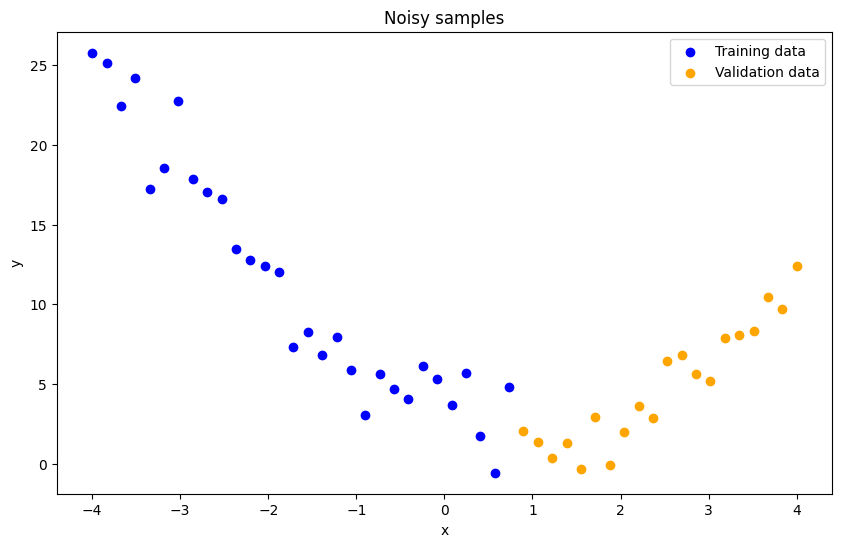
\includegraphics[width=0.5\textwidth]{pic/Polynomial_regression/noisy_samples.png}
        \end{center}
        \vfile
        \begin{center}
            Splitting samples to train and validation sets
        \end{center}
    \end{itemize}
\end{frame}

\begin{frame}{Quadratic regression vs Linear regression}
    \begin{minipage}{0.48\textwidth}
        \centering
        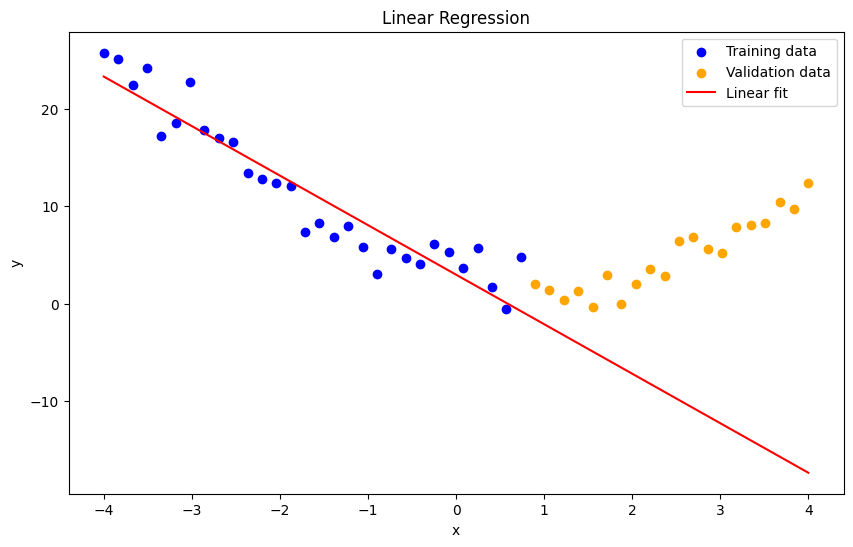
\includegraphics[width=0.95\textwidth]{pic/Polynomial_regression/linear_regression.png}
    \end{minipage} %
    \begin{minipage}{0.48\textwidth}
        \centering
        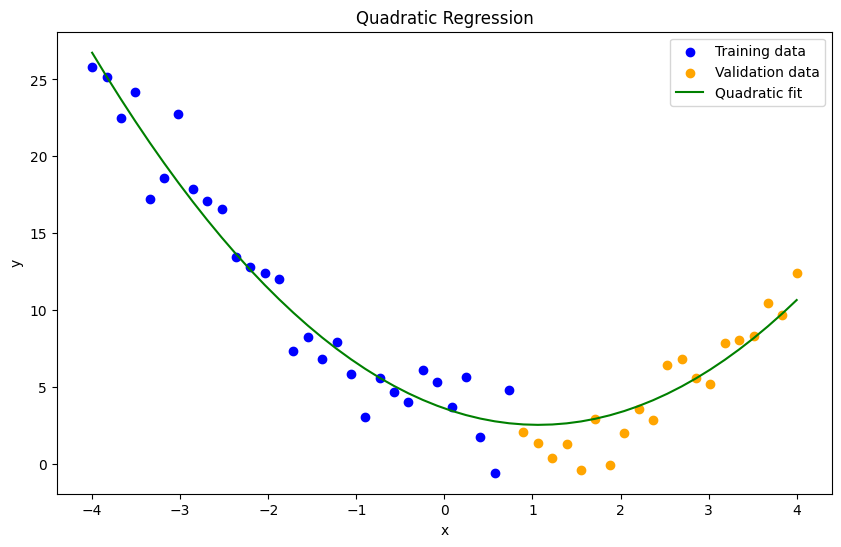
\includegraphics[width=0.95\textwidth]{pic/Polynomial_regression/quadratic_regression.png}
    \end{minipage}
    \vfile
    \begin{center}
        Fitting both quadratic and linear regression shows the power of polynomial regression on generalizing for more complex patterns.
    \end{center}
\end{frame}

% \begin{frame}{Polynomial Regression: Multivariate}
%     \begin{itemize}
%     \item  Given a feature vector \( \mathbf{x}^{(i)} = \left[ x_1^{(i)}, x_2^{(i)}, \dots, x_d^{(i)} \right] \) for the \( i \)-th data point, the hypothesis for multivariate polynomial regression is:
%     \[
%     h_\mathbf{w}(\mathbf{x}^{(i)}) = \hat{w}_0 + \sum_{j=1}^{d} \sum_{k=1}^{m} \hat{w}_k^{(j)} \left( x_j^{(i)} \right)^k
%     \]

%     where:
%     \begin{itemize}
%         \item \( \hat{w}_0 \) is the bias term.
%         \item \( \hat{w}_k^{(j)} \) represents the weight associated with the \( k \)-th power of the \( j \)-th feature.
%         \item \( m \) is the highest degree of the polynomial.
%         \item \( d \) is the number of features (dimension of \( \mathbf{x}^{(i)} \)).
%     \end{itemize}

%     \item
%     For a data point with two features \( x_1^{(i)} \) and \( x_2^{(i)} \), and a polynomial degree of \( 2 \) (quadratic), the hypothesis would be:

%     \[
%     h_\mathbf{w}(x_1^{(i)}, x_2^{(i)}) = \hat{w}_0 + \hat{w}_1^{(1)} x_1^{(i)} + \hat{w}_2^{(1)} \left( x_1^{(i)} \right)^2 + \hat{w}_1^{(2)} x_2^{(i)} + \hat{w}_2^{(2)} \left( x_2^{(i)} \right)^2
%     \]
%     \end{itemize}
% \end{frame}

% \begin{frame}{Polynomial Regression Analytical Solution: Multivariate}
%     \item Rewriting the SSE cost function using matrix form we have:
%     \[
%     J(\mathbf{w}) = \| \mathbf{y} - \mathbf{X'} \mathbf{w} \|_2^2
%     \]
%     \item \textbf{Analytical solution:} It has a closed form solution as:
%     \[
%     \hat{\mathbf{w}} = \left( \mathbf{X'}^T \mathbf{X'} \right)^{-1} \mathbf{X'}^T \mathbf{y}
%     \]
% \end{frame}



\begin{frame}{Generalization Overview}
    \textbf{Main Idea}: The ability of a model to perform well on unseen data
    \begin{itemize}
        \item \textbf{Training Set}: \( D = \{(x_i, y_i)\}_{i=1}^n \)
        \item \textbf{Test Set}: New data not seen during training
        \item \textbf{Cost Function}: Measures how well the model fits data
        \[
        J(w) = \sum_{i=1}^{n} (y^{(i)} - h_w(x^{(i)}))^2
        \]
        \item \textbf{Objective}: Minimize the cost function on unseen data (generalization error)
    \end{itemize}
\end{frame}

\begin{frame}{Expected Test Error}
    \textbf{Definition}: Expected performance on unseen data
    \begin{itemize}
        \item Test data sampled from the same distribution \( p(x, y) \)
        \[
        J(w) = \mathbb{E}_{p(x,y)}[(y - h_w(x))^2]
        \]
        \item Approximate using test set \( \hat{J}(w) \)
        \item Generalization error is the gap between training and test performance.
    \end{itemize}
\end{frame}

\begin{frame}{Training vs Test Error}
    \textbf{Key Concept}: Training error measures fit on known data, test error on unseen data
    \begin{itemize}
        \item \textbf{Training (empirical) error}:
        \[
        J_{\text{train}}(w) = \frac{1}{n} \sum_{i=1}^{n} \left( y^{(i)} - h_w(x^{(i)}) \right)^2
        \]
        \item \textbf{Test error}:
        \[
        J_{\text{test}}(w) = \frac{1}{m} \sum_{i=1}^{m} \left(y_{\text{test}}^{(i)} - h_w(x_{\text{test}}^{(i)})\right)^2
        \]
        \item \textbf{Goal}: Minimize the test error (generalization).
    \end{itemize}
\end{frame}

\begin{frame}{Overfitting Definition}
    \textbf{Concept}: A model fits the training data well but performs poorly on the test set
    \[
    J_{\text{train}}(w) \ll J_{\text{test}}(w)
    \]
    \begin{itemize}
        \item Causes: Model too complex, high variance
        \item Consequence: Captures noise in training data, fails on unseen data
    \end{itemize}
\end{frame}



\begin{frame}{Underfitting Definition}
    \textbf{Concept}: The model is too simple and cannot capture the structure of the data
    \[
    J_{\text{train}}(w) \approx J_{\text{test}}(w) \gg 0
    \]
    \begin{itemize}
        \item Causes: Model lacks complexity, high bias
        \item Consequence: Poor fit on both training and test data
    \end{itemize}
\end{frame}



\begin{frame}{Regime 1: High Variance}
\centering
\renewcommand{\arraystretch}{1.3}
\begin{tabular}{|p{0.9\linewidth}|}
\hline
\textbf{Cause:} Poor performance due to high variance. \\ \hline

\textbf{Symptoms:}
\begin{itemize}
    \item Training error $\ll$ Test error
    \item Training error $<$ $\epsilon$
    \item Test error $>$ $\epsilon$
\end{itemize} \\ \hline

\textbf{Remedies:}
\begin{itemize}
    \item Add more training data
    \item Reduce model complexity (simpler models are less prone to high variance)
    \item Use Bagging (covered later)
\end{itemize} \\ \hline
\end{tabular}


\vspace{0.3cm}
\textit{Note:} $\epsilon$ is a predefined threshold for acceptable training error.
\end{frame}


\begin{frame}{Regime 2: High Bias}
\centering
\renewcommand{\arraystretch}{1.3}
\begin{tabular}{|p{0.9\linewidth}|}
\hline
\textbf{Cause:} The model is too simple and underfits the data. \\ \hline

\textbf{Symptoms:}
\begin{itemize}
    \item Training error $>$ $\epsilon$
\end{itemize} \\ \hline

\textbf{Remedies:}
\begin{itemize}
    \item Use a more complex model (e.g., kernelized or non-linear)
    \item Add more features
    \item Apply Boosting (covered later)
\end{itemize} \\ \hline
\end{tabular}
\end{frame}





\begin{frame}{Generalization: polynomial regression}
    \begin{minipage}{0.45\textwidth}
        \centering
        \begin{figure}[h]
        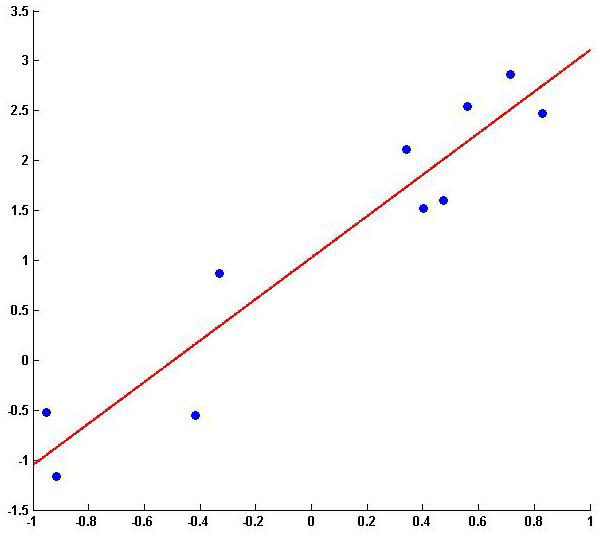
\includegraphics[width=0.8\textwidth]{pic/Polynomial_regression/degree_1.png}
        \end{figure}
        \begin{center}
            Degree of 1
        \end{center}
    \end{minipage}%
    \begin{minipage}{0.45\textwidth}
        \centering
        \begin{figure}[h]
        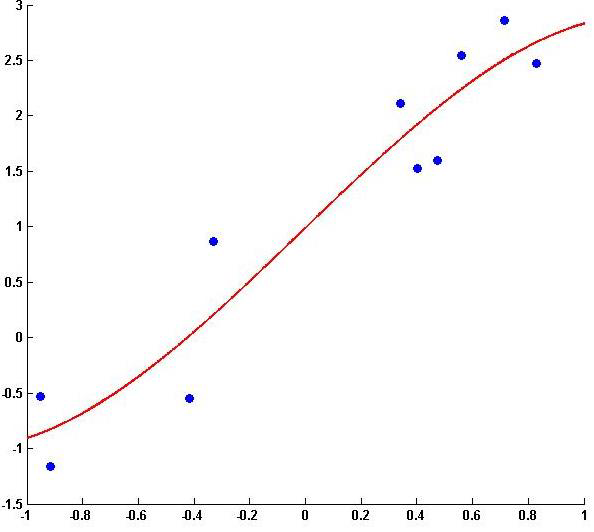
\includegraphics[width=0.8\textwidth]{pic/Polynomial_regression/degree_3.png}
        \end{figure}
        \begin{center}
            Degree of 3
        \end{center}
    \end{minipage}
    \vfill
    \begin{tikzpicture}[remember picture,overlay]
        \node[anchor=south west, xshift=0.1cm, yshift=0.22cm] at (current page.south west) {
            \scriptsize Example adapted from slides of Dr. Soleymani, ML course, Sharif University of technology.
        };
    \end{tikzpicture}
    % \vfill
    % \begin{center}
    %     \tiny Example adapted from slides of Dr. Soleymani, Machine Learning course, Sharif University of technology.
    % \end{center}
\end{frame}

\begin{frame}{Overfitting: polynomial regression}
    \begin{minipage}{0.45\textwidth}
        \centering
        \begin{figure}[h]
        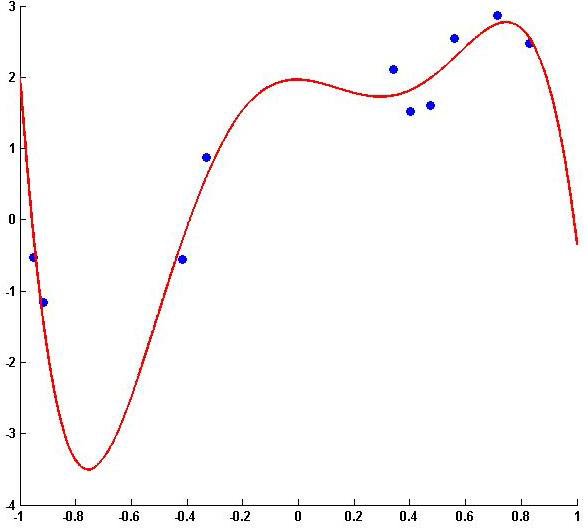
\includegraphics[width=0.8\textwidth]{pic/Polynomial_regression/degree_5.png}
        \end{figure}
        \begin{center}
            Degree of 5
        \end{center}
    \end{minipage}%
    \begin{minipage}{0.45\textwidth}
        \centering
        \begin{figure}[h]
        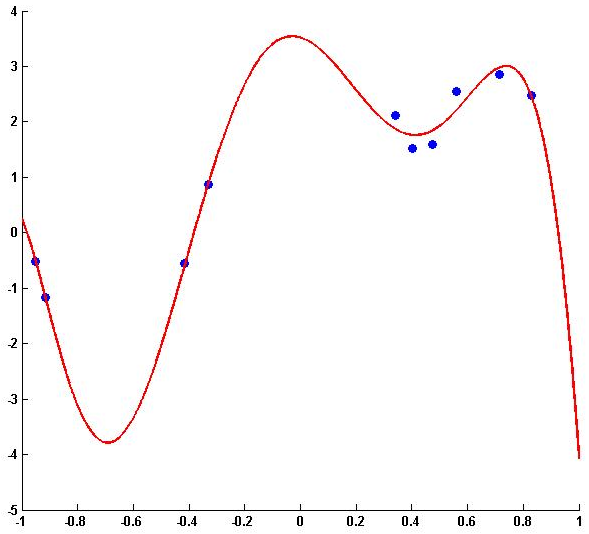
\includegraphics[width=0.8\textwidth]{pic/Polynomial_regression/degree_7.png}
        \end{figure}
        \begin{center}
            Degree of 7
        \end{center}
    \end{minipage}
    \vfill
    \begin{tikzpicture}[remember picture,overlay]
        \node[anchor=south west, xshift=0.1cm, yshift=0.22cm] at (current page.south west) {
            \scriptsize Example adapted from slides of Dr. Soleymani, ML course, Sharif University of technology.
        };
    \end{tikzpicture}
\end{frame}

% \begin{frame}{Example: Regression using polynomial curve}
% \begin{minipage}{0.45\textwidth}
%         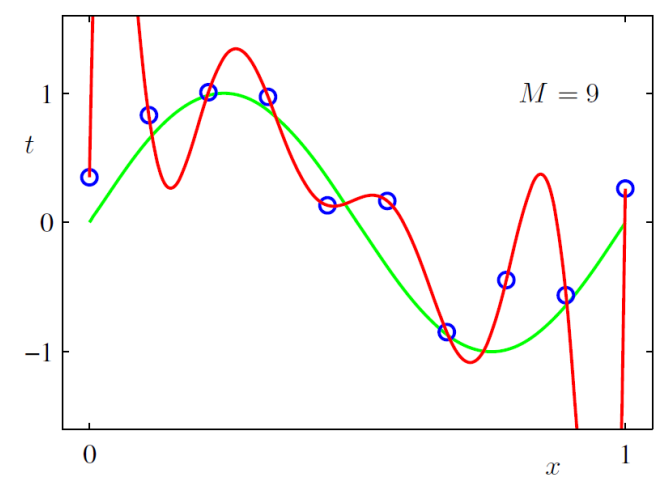
\includegraphics[width=\linewidth]{pic/10.png}
%         \captionof{Figure adapted from Machine Learning and Pattern Recognition, Bishop.}
%     \end{minipage}%
% \begin{minipage}{0.3\textwidth}
%     \vspace{0.5cm} % Adjust vertical alignment of the text if needed
%     \begin{itemize}
%             \item \[t = \sin(2 \pi x) + \epsilon\]
%         \end{itemize}
% \end{minipage}
% \end{frame}

\begin{frame}{Polynomial regression with various degrees: example}
    \begin{minipage}{0.95\textwidth}
        \centering
        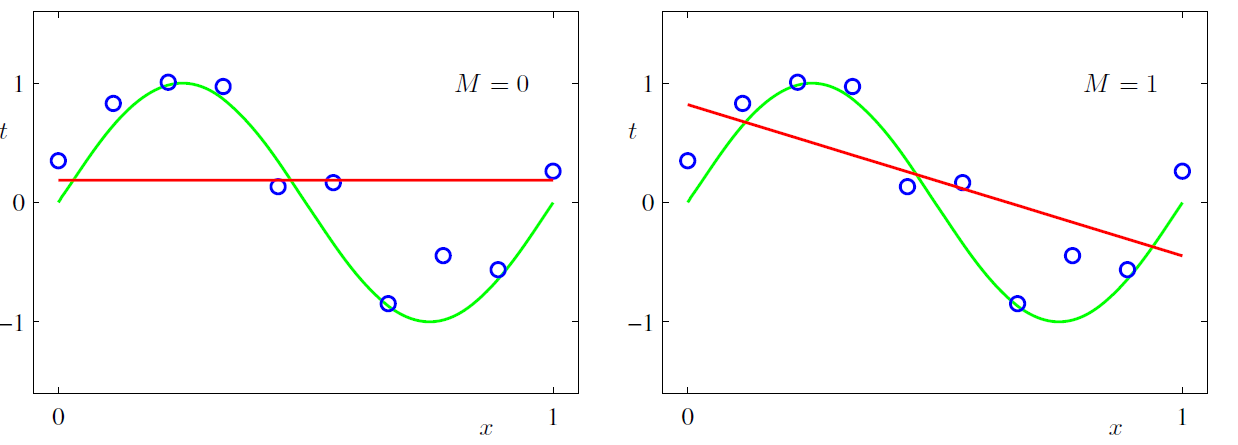
\includegraphics[width=1\textwidth]{pic/Polynomial_regression/pr_low_degrees.png}
    \end{minipage}
    % \vfill
    % \[ t = sin(2\pi x) + \epsilon \]
    % \vfill
    % \begin{center}
    %     \tiny Figures adapted from Machine Learning and Pattern Recognition, Bishop
    % \end{center}
    \vfill
    \begin{tikzpicture}[remember picture,overlay]
        \node[anchor=south west, xshift=0.1cm, yshift=0.22cm] at (current page.south west) {
            \scriptsize Figures adapted from Machine Learning and Pattern Recognition, Bishop
        };
    \end{tikzpicture}
\end{frame}

\begin{frame}{Polynomial regression with various degrees: example (cont.)}
    \begin{minipage}{0.95\textwidth}
        \centering
        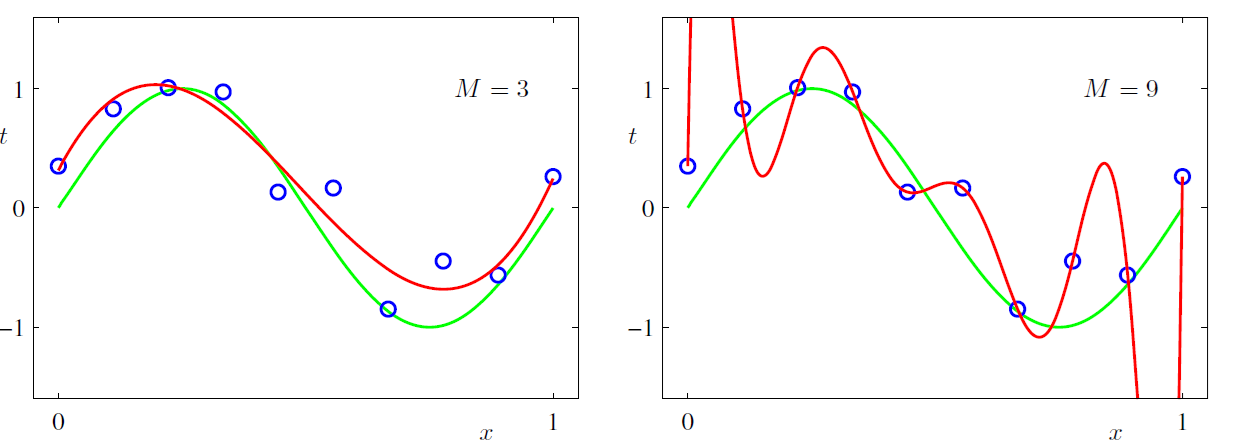
\includegraphics[width=1\textwidth]{pic/Polynomial_regression/pr_high_degrees.png}
    \end{minipage}
    % \vfill
    % \[ t = sin(2\pi x) + \epsilon \]
    % \vfill
    % \begin{center}
    %     \tiny Figures adapted from Machine Learning and Pattern Recognition, Bishop
    % \end{center}
    \vfill
    \begin{tikzpicture}[remember picture,overlay]
        \node[anchor=south west, xshift=0.1cm, yshift=0.22cm] at (current page.south west) {
            \scriptsize Figures adapted from Machine Learning and Pattern Recognition, Bishop
        };
    \end{tikzpicture}
\end{frame}

\begin{frame}{Root mean squared error}
    \begin{minipage}{0.45\textwidth}
        \centering
        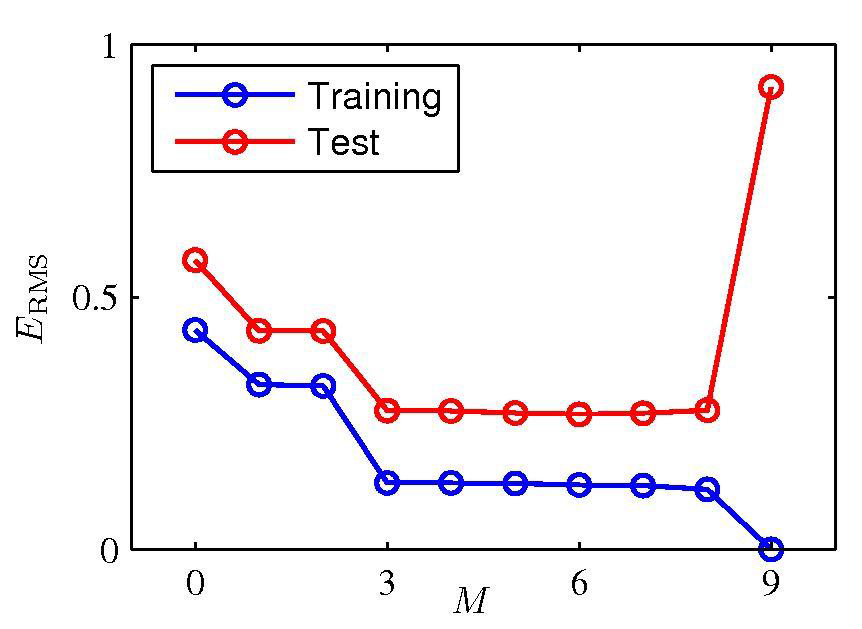
\includegraphics[width=0.9\textwidth]{pic/Polynomial_regression/erms_polynomial_regression.png}
    \end{minipage}%
    \begin{minipage}{0.45\textwidth}
        \[
        E_{RMS} = \sqrt{\dfrac{\sum_{i=1}^n \left( y^{(i)} - f(\mathbf{x}^{(i)}; \mathbf{w} \right)^2}{n}}
        \]
    \end{minipage}
    % \vfill
    % \begin{center}
    %     \tiny Figure adapted from Machine Learning and Pattern Recognition, Bishop
    % \end{center}
    \vfill
    \begin{tikzpicture}[remember picture,overlay]
        \node[anchor=south west, xshift=0.1cm, yshift=0.22cm] at (current page.south west) {
            \scriptsize Figures adapted from Machine Learning and Pattern Recognition, Bishop
        };
    \end{tikzpicture}
\end{frame}

\begin{frame}{Bias-Variance Decomposition}
    \textbf{Generalization error decomposition}:
    \[
    \mathbb{E}[(y - h_w(x))^2] = (\text{Bias})^2 + \text{Variance} + \text{Noise}
    \]
    \begin{itemize}
        \item \textbf{Bias}: Error due to simplifying assumptions in the model
        \[
        \text{Bias}(x) = \mathbb{E}[h_w(x)] - f(x)
        \]
        \item \textbf{Variance}: Sensitivity of the model to training data
        \[
        \text{Variance}(x) = \mathbb{E}[(h_w(x) - \mathbb{E}[h_w(x)])^2]
        \]
        \item \textbf{Noise}: Irreducible error from the inherent randomness in data
    \end{itemize}
\end{frame}

\begin{frame}{High Bias in Simple Models}
    \textbf{Explanation}: Simple models, such as linear regression, often underfit
    \[
    h_w(x) = w_0 + w_1 x
    \]
    \begin{itemize}
        \item Bias remains large even with infinite data
        \[
        \text{Bias}^2 \gg \text{Variance}
        \]
        \item Leads to large generalization error
    \end{itemize}
\end{frame}

\begin{frame}{High Variance in Complex Models}
    \textbf{Explanation}: Complex models tend to overfit
    \[
    h_w(x) = w_0 + w_1 x + w_2 x^2 + \dots + w_m x^m
    \]
    \begin{itemize}
        \item Variance dominates when the model is too complex
        \[
        \text{Variance} \gg \text{Bias}
        \]
        \item Fits noise, leading to high test error
    \end{itemize}
\end{frame}

\begin{frame}{Bias-Variance Tradeoff}
    \textbf{Tradeoff}: Balancing between bias and variance is key for optimal performance
    \begin{itemize}
        \item Low complexity: High bias, low variance
        \item High complexity: Low bias, high variance
    \end{itemize}
    \[
    % \text{Generalization error} = (\text{Bias})^2 + \text{Variance} + \text{Noise}
    \]
    \begin{center}
    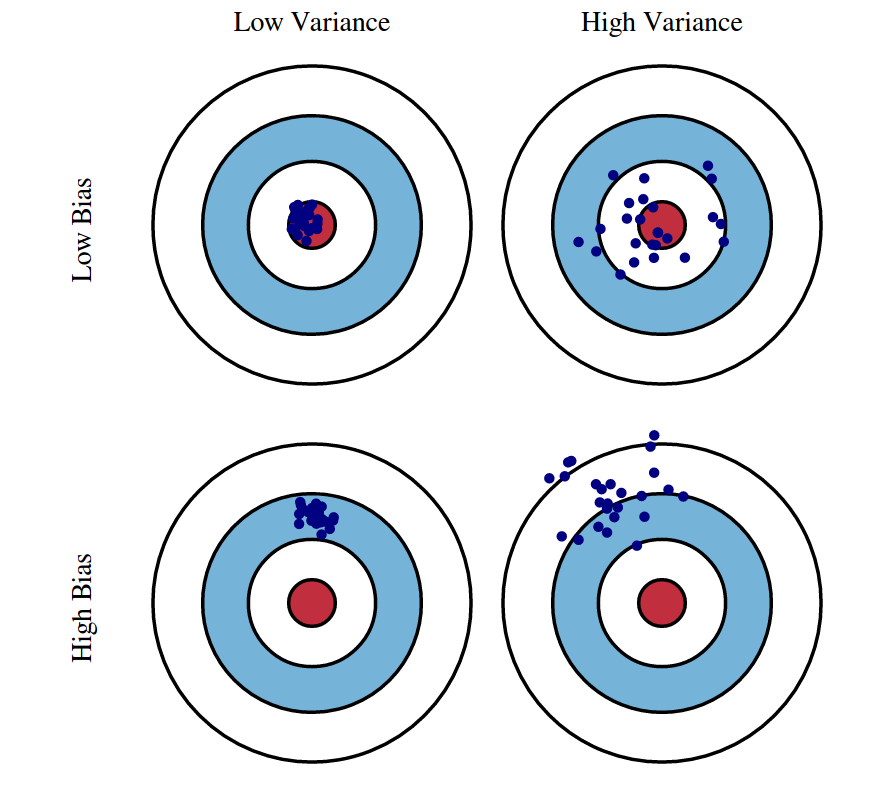
\includegraphics[width=0.35\linewidth]{pic/bias-variance.png}
    \hspace{0.25cm}
    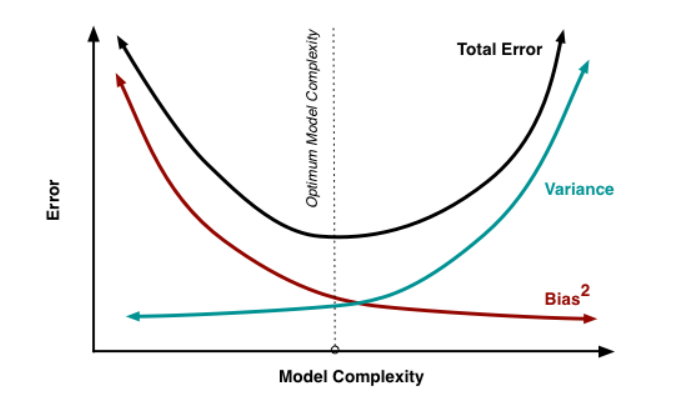
\includegraphics[width=0.5\linewidth]{pic/bias-variance2.png}
 \end{center}

\end{frame}

\begin{frame}{Regularization}
    \textbf{Purpose}: Prevent overfitting by penalizing large weights
    \[
    J_{\lambda}(w) = J(w) + \lambda R(w)
    \]
    \begin{itemize}
        % \item Common regularizer: \( R(w) = ||w||_2^2 \) (L2 norm)
        \item Common regularizers: L1 and L2 norms
        \item \( \lambda \) controls the balance between fit and simplicity
    \end{itemize}
\end{frame}

\begin{frame}{Effect of Regularization Parameter \( \lambda \)}
    \textbf{Balancing Fit and Complexity}:
    \[
    J_{\lambda}(w) = J(w) + \lambda \sum_{j=1}^{m} w_j^2 = J(w) + \lambda \mathbf{w}^T\mathbf{w}
    \]
    \begin{itemize}
        \item Large \( \lambda \): Forces smaller weights, reduces complexity, increases bias, decreases variance
        \item Small \( \lambda \): Allows larger weights, increases complexity, reduces bias, increases variance
    \end{itemize}
\end{frame}

\begin{frame}{Effect of Regularization parameter \( \lambda \)}
    \begin{minipage}{0.32\textwidth}
        \centering
        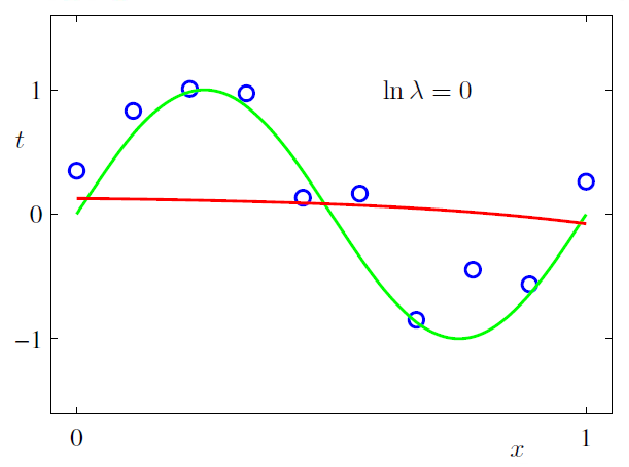
\includegraphics[width=1.0\textwidth]{pic/Regularization/regularization_0.png}
    \end{minipage} %
    \begin{minipage}{0.32\textwidth}
        \centering
        \includegraphics[width=1.0\textwidth]{pic/Regularization/regularization_18.png}
    \end{minipage} %
    \begin{minipage}{0.32\textwidth}
        \centering
        \includegraphics[width=1.0\textwidth]{pic/Regularization/regularization_inf.png}
    \end{minipage}
    \vfill
    \[
    J_{\lambda}(w) = \sum_{i=1}^n \left( t^{(i)} - f(\mathbf{x}^{(i)}; \mathbf{w}) \right)^2 + \lambda \mathbf{w}^T\mathbf{w}
    \]
    \[
    f(\mathbf{x}^{(n)}; \mathbf{w}) = w_0 + w_1 x + \dots + w_9 x^9
    \]
    % \vfill
    % \begin{center}
    %     \tiny Figures adapted from Machine Learning and Pattern Recognition, Bishop.
    % \end{center}
    \vfill
    \begin{tikzpicture}[remember picture,overlay]
        \node[anchor=south west, xshift=0.1cm, yshift=0.22cm] at (current page.south west) {
            \scriptsize Figures adapted from Machine Learning and Pattern Recognition, Bishop
        };
    \end{tikzpicture}
\end{frame}

\begin{frame}{Effect of regularization on weights}
    \begin{minipage}{0.9\textwidth}
        \centering
        \includegraphics[width=0.7\textwidth]{pic/Regularization/weights.png}
    \end{minipage}
    % \vfill
    % \begin{center}
    %     \tiny Figure adapted from Machine Learning and Pattern Recognition, Bishop.
    % \end{center}
    \vfill
    \begin{tikzpicture}[remember picture,overlay]
        \node[anchor=south west, xshift=0.1cm, yshift=0.22cm] at (current page.south west) {
            \scriptsize Table adapted from Machine Learning and Pattern Recognition, Bishop
        };
    \end{tikzpicture}
\end{frame}

\begin{frame}{Regularization parameter}
    \begin{minipage}{0.45\textwidth}
    \centering
    \includegraphics[width=1\textwidth]{pic/Regularization/regularization_parameter_erms.png}
    \end{minipage} %
    \begin{minipage}{0.45\textwidth}
    \begin{itemize}
        \item \( \lambda \) controls the effective complexity of the model
        \item hence the degree of overfitting
    \end{itemize}
    \end{minipage}
    % \vfill
    % \begin{center}
    %     \tiny Figure adapted from Machine Learning and Pattern Recognition, Bishop.
    % \end{center}
    \vfill
    \begin{tikzpicture}[remember picture,overlay]
        \node[anchor=south west, xshift=0.1cm, yshift=0.22cm] at (current page.south west) {
            \scriptsize Figures adapted from Machine Learning and Pattern Recognition, Bishop
        };
    \end{tikzpicture}
\end{frame}



% \section{Cross-validation}
% \begin{frame}{Cross-Validation Concept}
%     \textbf{Purpose}: Estimate model performance and prevent overfitting
%     \[
%     J_v(w) = \frac{1}{v_{\text{set}}} \sum_{i \in v_{\text{set}}} (y_i - h_w(x^{(i)}))^2
%     \]
%     \begin{itemize}
%         \item Use validation error \( J_v(w) \) to select the best model
%     \end{itemize}
% \end{frame}

% \begin{frame}{k-Fold Cross-Validation (CV)}
%     \textbf{k-Fold Procedure}:
%     \[
%     \text{For each } i = 1 \text{ to } k, \text{train on all except } i\text{-th part, validate on } i\text{-th part.}
%     \]
%     \begin{itemize}
%         \item Average performance across \( k \) runs
%         \item Common choices: \( k = 5 \), \( k = 10 \)
%     \end{itemize}
% \end{frame}

\begin{frame}{Introduction to Regression (Probabilistic Perspective)}
    \begin{itemize}
        \item \textbf{Objective:} Model the relationship between input \( \mathbf{x} \) and output \( y \).
        \item \textbf{Uncertainty:} Output \( y \) has an associated uncertainty modeled by a probability distribution.
        \item \textbf{Example:}
        \[
        y = f(\mathbf{x}; \mathbf{w}) + \epsilon \quad , \quad \epsilon \sim \mathcal{N}(0, \sigma^2)
        \]
        \item The goal is to learn \( f(\mathbf{x}; \mathbf{w}) \) to predict \( y \).
    \end{itemize}
\end{frame}

\begin{frame}{Curve Fitting with Noise}
    \begin{itemize}
        \item In real-world scenarios, observed output \( y \) is noisy.
        \item \textbf{Model: True output plus noise}
        % \[
        % y = f(\mathbf{x}; \mathbf{w}) + \epsilon, \quad \epsilon \sim \mathcal{N}(0, \sigma^2)
        % \]
        \[
        y = f(\mathbf{x}; \mathbf{w}) + \epsilon
        \]
        \item Noise represents unknown or unmodeled factors.
        \item \textbf{Example:} Predicting house prices based on features with inherent unpredictability.
    \end{itemize}
\end{frame}

\begin{frame}{Expected Value of Output}
    \begin{itemize}
        \item Best Estimate: The conditional expectation of \( y \) given \( \mathbf{x} \).
        \[
        \mathbb{E}[y | \mathbf{x}] = f(\mathbf{x}; \mathbf{w})
        \]
        \item Goal: Learn a function \( f(\mathbf{x}; \mathbf{w}) \) that represents the average behavior of the data.
        \item Key Point: The model captures the mean of the target variable given input \( \mathbf{x} \).
    \end{itemize}
\end{frame}

\begin{frame}{Maximum Likelihood Estimation (MLE)}
    \begin{itemize}
        \item \textbf{MLE:} A method to estimate parameters that maximize the likelihood of the data.
        \item Given data \( \mathcal{D} = \{ (\mathbf{x}_i, y_i) \}_{i=1}^n \), MLE maximizes:
        \[
        L(\mathcal{D}; \mathbf{w}, \sigma^2) = \prod_{i=1}^n p(y_i | \mathbf{x}_i, \mathbf{w}, \sigma^2)
        \]
        \item MLE finds parameters \( \mathbf{w} \) and \( \sigma^2 \) that best explain the data.
    \end{itemize}
\end{frame}

\begin{frame}{Maximum Likelihood Estimation (cont.)}
    \begin{itemize}
        \item Instead of maximizing the likelihood, it is often easier to maximize the log-likelihood:
        \[
        \log L(\mathcal{D}; \mathbf{w}, \sigma^2) = \sum_{i=1}^n \log  p(y_i | \mathbf{x}_i, \mathbf{w}, \sigma^2)
        \]
        \item It is because \( \log f(x) \) preserves the behaviour of \( f(x) \).
        \item It is also easier to find derivative on summation of terms.
    \end{itemize}
\end{frame}

\begin{frame}{Univariate Linear Function Example}
    \begin{itemize}
        \item Assuming Gaussian noise with parameters \( (0, \sigma^2) \), probability of observing real output value \( y \) is:
        \[
        p(y | \mathbf{x}, \mathbf{w}, \sigma^2) = \frac{1}{\sqrt{2\pi \sigma^2}} \exp \left( - \frac{(y - f(\mathbf{x}; \mathbf{w}))^2}{2\sigma^2} \right)
        \]

        \item For a simple linear model \( f(\mathbf{x}; \mathbf{w}) = w_0 + w_1 x \) we have:
        \[
        p(y | x, \mathbf{w}, \sigma^2) = \frac{1}{\sqrt{2\pi \sigma^2}} \exp \left( - \frac{(y - w_0 - w_1 x)^2}{2\sigma^2} \right)
        \]
        % \item MLE Objective: Maximize the likelihood of the data points fitting the model.
        \item \textbf{Key Observation:} Points far from the fitted line will have a low likelihood value.
    \end{itemize}
\end{frame}

\begin{frame}{Log-Likelihood and Sum of Squares}
    \begin{itemize}
        \item Using log-likelihood we have:
        \[
        \log L(\mathcal{D}; \mathbf{w}, \sigma^2) = -n \log \sigma - \frac{n}{2} \log(2\pi) - \frac{1}{2\sigma^2} \sum_{i=1}^n (y^{(i)} - f(\mathbf{x}^{(i)}; \mathbf{w}))^2
        \]
        \item Since the objective of MLE is to optimize with regards to random variables, we can rule out the constants:
        \[
        \log L(\mathcal{D}; \mathbf{w}, \sigma^2) \sim - \sum_{i=1}^n (y^{(i)} - f(\mathbf{x}^{(i)}; \mathbf{w}))^2
        \]
        \item \textbf{Equivalence:} Maximizing the log-likelihood is equivalent to minimizing the Sum of Squared Errors (SSE):
        \[
        J(\mathbf{w}) = \sum_{i=1}^n (y^{(i)} - f(\mathbf{x}^{(i)}; \mathbf{w}))^2
        \]
    \end{itemize}
\end{frame}

\begin{frame}{Estimating \( \sigma^2 \)}
    \begin{itemize}
        \item The maximum likelihood estimate of the noise variance \( \sigma^2 \):
        \[
        \hat{\sigma}^2 = \frac{1}{n} \sum_{i=1}^n \left( y^{(i)} - f(\mathbf{x}^{(i)}; \hat{\mathbf{w}}) \right)^2
        \]
        \item Interpretation: Mean squared error of the predictions.
        \item Note: \( \sigma^2 \) reflects the noise level in the observations.
    \end{itemize}
\end{frame}

\begin{frame}{Maximum A Posteriori Estimation (MAP)}
    \begin{itemize}
        \item \textbf{MAP:} Estimate parameters by maximizing the posterior:
        \[
            \mathbf{w}_{\text{MAP}}
            = \arg\max_{\mathbf{w}}  p(\mathbf{w}\mid \mathcal{D})
            \propto \arg\max_{\mathbf{w}}  \prod_{i=1}^n p(y_i\mid \mathbf{x}_i,\mathbf{w},\sigma^2)\, p(\mathbf{w})
        \]
        \item Equivalently, maximize the log-posterior:
        \[
            \mathbf{w}_{\text{MAP}}
            = \arg\max_{\mathbf{w}}  \sum_{i=1}^n \log p(y_i\mid \mathbf{x}_i,\mathbf{w},\sigma^2) + \log p(\mathbf{w})
        \]
        \item
        In MAP with a prior, large datasets wash out the prior, so the posterior effectively matches the data-only estimate (\(\approx\) MLE).

        \item When data are scarce, the prior injects knowledge that shapes the posterior, making MAP meaningfully different from MLE.
    \end{itemize}
\end{frame}

\begin{frame}{MAP with a Gaussian Prior}
    \begin{itemize}
        \item \textbf{Prior (additional assumption):} \(\mathbf{w}\sim \mathcal{N}(\mathbf{0},\tau^2\mathbf{I})\)
        \[
            p(\mathbf{w})=\frac{1}{\sqrt{2\pi\tau^2}}
            \exp\!\left(-\frac{\mathbf{w}^\top \mathbf{w}}{2\tau^2}\right)
        \]
        \item With Gaussian noise \(y_i = \mathbf{x}_i^\top \mathbf{w} + \varepsilon_i, \varepsilon_i\sim\mathcal{N}(0,\sigma^2)\),
        maximizing the log-posterior is (up to constants) equivalent to:
        \[
            \arg\min_{\mathbf{w}}
            \frac{1}{2\sigma^2}\sum_{i=1}^n (y_i-\mathbf{x}_i^\top\mathbf{w})^2
            + \frac{1}{2\tau^2}\,\|\mathbf{w}\|_2^2
        \]
        \item Defining \(\displaystyle \lambda=\frac{\sigma^2}{n\tau^2}\), the MAP objective becomes
        \[
            J_{\text{MAP}}(\mathbf{w})
            = \frac{1}{n}\sum_{i=1}^n (y_i-\mathbf{x}_i^\top\mathbf{w})^2 + \lambda \|\mathbf{w}\|_2^2
        \]
        \item \textbf{Equivalence:} This is Ridge (Regularized) Regression.
    \end{itemize}
\end{frame}


% \begin{frame}{Maximum a Posteriori (MAP) Estimation}
%     \begin{itemize}
%         \item \textbf{MAP:} Incorporates \textbf{prior information} about parameters.
%         \[
%         \mathbf{w}_{MAP} = \arg \max_{\mathbf{w}} p(\mathbf{w} | \mathcal{D}) = \arg \max_{\mathbf{w}} p(\mathcal{D} | \mathbf{w}) p(\mathbf{w})
%         \]
%         \item Prior Distribution:
%         \[
%         p(\mathbf{w}) = \mathcal{N}(0, \alpha^2 I)
%         \]
%         \item Posterior Distribution:
%         \[
%         p(\mathbf{w} | \mathcal{D})
%         \]
%         \item Key Difference: Unlike MLE, MAP includes a prior to regularize the solution.
%     \end{itemize}
% \end{frame}

% \begin{frame}{MAP as Regularized Least Squares}
%     \begin{itemize}
%         \item MAP estimation is equivalent to minimizing a regularized SSE:
%         \[
%         \mathbf{w}_{MAP} = \arg \min_{\mathbf{w}} \frac{1}{\sigma^2} \sum_{i=1}^n (y_i - f(\mathbf{x}_i; \mathbf{w}))^2 + \frac{1}{\alpha^2} \mathbf{w}^\top \mathbf{w}
%         \]
%         \item Regularization Term: \( \lambda = \frac{\sigma^2}{\alpha^2} \) controls how strongly the model is regularized.
%     \end{itemize}
% \end{frame}

% \begin{frame}{Bayesian Approach}
%     \begin{itemize}
%         \item The Bayesian approach integrates over the distribution of parameters:
%         \[
%         p(y | \mathbf{x}, \mathcal{D}) = \int p(y | \mathbf{x}, \mathbf{w}) p(\mathbf{w} | \mathcal{D}) d\mathbf{w}
%         \]
%         \item This approach incorporates uncertainty in the parameters into the predictions.
%         \item Benefit: Provides a probabilistic interpretation of the model’s predictions.
%     \end{itemize}
% \end{frame}

% \begin{frame}{Predictive Distribution}
%     \begin{itemize}
%         \item In Bayesian linear regression, the predictive distribution is Gaussian:
%         \[
%         p(y | \mathbf{x}, \mathcal{D}) = \mathcal{N}(m_N^\top \mathbf{x}, \sigma_N^2(\mathbf{x}))
%         \]
%         \item \( m_N \): Posterior mean.
%         \item \( \sigma_N^2(\mathbf{x}) \): Predictive variance.
%         \item Key Point: This captures both the prediction and the uncertainty around it.
%     \end{itemize}
% \end{frame}

% \begin{frame}{Prior and Posterior Distributions}
%     \begin{itemize}
%         \item Prior: Before seeing data, we assume a prior distribution on \( \mathbf{w} \):
%         \[
%         p(\mathbf{w}) = \mathcal{N}(0, \alpha^2 I)
%         \]
%         \item Posterior: After observing data, we compute the posterior distribution \( p(\mathbf{w} | \mathcal{D}) \).
%         \item Bayesian Prediction: Integrates over the posterior to account for uncertainty.
%     \end{itemize}
% \end{frame}

% \begin{frame}{Example of Predictive Distribution}
% \small Example: Sinusoidal data with 9 Gaussian basis functions.

% \vspace{0.3cm}
% \begin{minipage}{0.65\textwidth}
%     \centering
%     \includegraphics[width=0.9\textwidth]{pic/9.png}
%     \caption{\scriptsize \textit{Figure adapted from Machine Learning and Pattern Recognition, Bishop.}}
% \end{minipage}%
% \begin{minipage}{0.3\textwidth}
%     \vspace{0.5cm} % Adjust vertical alignment of the text if needed
%     \begin{itemize}
%         \item \textbf{Red curve}: Mean of the predictive distribution.
%         \item \textbf{Pink region}: One standard deviation from the mean.
%     \end{itemize}
% \end{minipage}
% \end{frame}






\begin{frame}{Contributions}
\begin{itemize}
\item \textbf{This slide has been prepared thanks to:}
\begin{itemize}
    \setlength{\itemsep}{10pt} % Adjust the value to control the spacing
    \item \href{https://github.com/AidaJalali}{Aida Jalali}
    \item \href{https://github.com/alirezamirrokni}{Alireza Mirrokni}
    \item \href{https://silentdrift.github.io/}{Arshia Gharooni}
    \item \href{https://github.com/Mahan-Bayhaghi}{Mahan Bayhaghi}


\end{itemize}
\end{itemize}

\end{frame}

\begin{frame}[allowframebreaks]
    \bibliography{ref}
    \bibliographystyle{ieeetr}
    \nocite{*}
\end{frame}


\end{document}








